\documentclass[a4paper,12pt]{report}
\usepackage{fontspec}
\usepackage{polyglossia}
\setdefaultlanguage{slovak}
\usepackage{amsmath, amssymb, amsthm}
%\usepackage[utf8]{inputenc}
\usepackage{graphicx}
\usepackage{pdfpages}

\usepackage{lmodern}
\usepackage{microtype}
\usepackage{booktabs}
%\usepackage{concmath}
%\usepackage[T1]{fontspec}

\usepackage{setspace}
\usepackage{caption}
\usepackage{url}
\usepackage{siunitx} %si units
\usepackage[left=3.5cm, right=2.0cm, top=2.5cm, bottom=2.5cm]{geometry}

\usepackage[export]{adjustbox}% http://ctan.org/pkg/adjustbox

\usepackage[backend=bibtex, natbib=true, style=alphabetic]{biblatex}
\addbibresource{literatura.bib}

\usepackage{listings}
\usepackage{color}

\renewcommand{\lstlistingname}{Ukážka kódu}

\definecolor{dkgreen}{rgb}{0,0.6,0}
\definecolor{gray}{rgb}{0.5,0.5,0.5}
\definecolor{mauve}{rgb}{0.58,0,0.82}
\definecolor{myyellow}{rgb}{1, 1, 0.9}

\usepackage{float}
\floatstyle{boxed}
\AtBeginDocument{\addtocontents{toc}{\protect\thispagestyle{empty}}} 

\usepackage[bookmarks, pdftitle={Využitie oklúzie v rozšírenej realite}, pdfauthor={Viktor Seč}, pdfsubject={Bakalárska práca}, pdfkeywords={rozšírená realita, počítačové videnie, rozpoznávanie markerov, oklúzia},hidelinks]{hyperref}

\setlength{\parskip}{1em}

%\include{csprimes}
\date{\today}
%\begin{comment}
\makeatletter
\renewcommand*\@makechapterhead[1]{%
  %\vspace*{50\p@}%
  {\parindent \z@ \raggedright \normalfont
    \ifnum \c@secnumdepth >\m@ne
        \huge\bfseries \@chapapp\space \thechapter
        \par\nobreak
        \vskip 20\p@
    \fi
    \interlinepenalty\@M
    \Huge \bfseries #1\par\nobreak
    \vskip 40\p@
  }}

\makeatother
%\end{comment}

\usepackage{caption}

\begin{document}
\pagenumbering{gobble}
\thispagestyle{empty}
\onehalfspacing

{\Large
\centerline{\textbf{Univerzita Komenského v Bratislave}}
\centerline{\textbf{Fakulta Matematiky, Fyziky a Informatiky}}
}

\vfil
\vspace{\stretch{1}}
  \begin{center}
    {\LARGE \textbf{Využitie oklúzie v rozšírenej realite}}
    
    \bigskip
    \bigskip

    {\Large Bakalárska práca}\\
  \end{center}
  \vfil

\vspace{\stretch{1}}
\noindent
\begin{tabular}[B]{ll}
Študijný program: & aplikovaná informatika \\
Študijný odbor: & aplikovaná informatika (2511) \\
Školiace pracovisko: & Katedra aplikovanej informatiky \\
Školiteľ:  & RNDr. Zuzana Berger Haladová, PhD. \\
\end{tabular}

\bigskip

\vspace{\stretch{0.1}}
\noindent
\textbf{Bratislava, 2015} \hfill \textbf{Viktor Seč} 	
\pagebreak

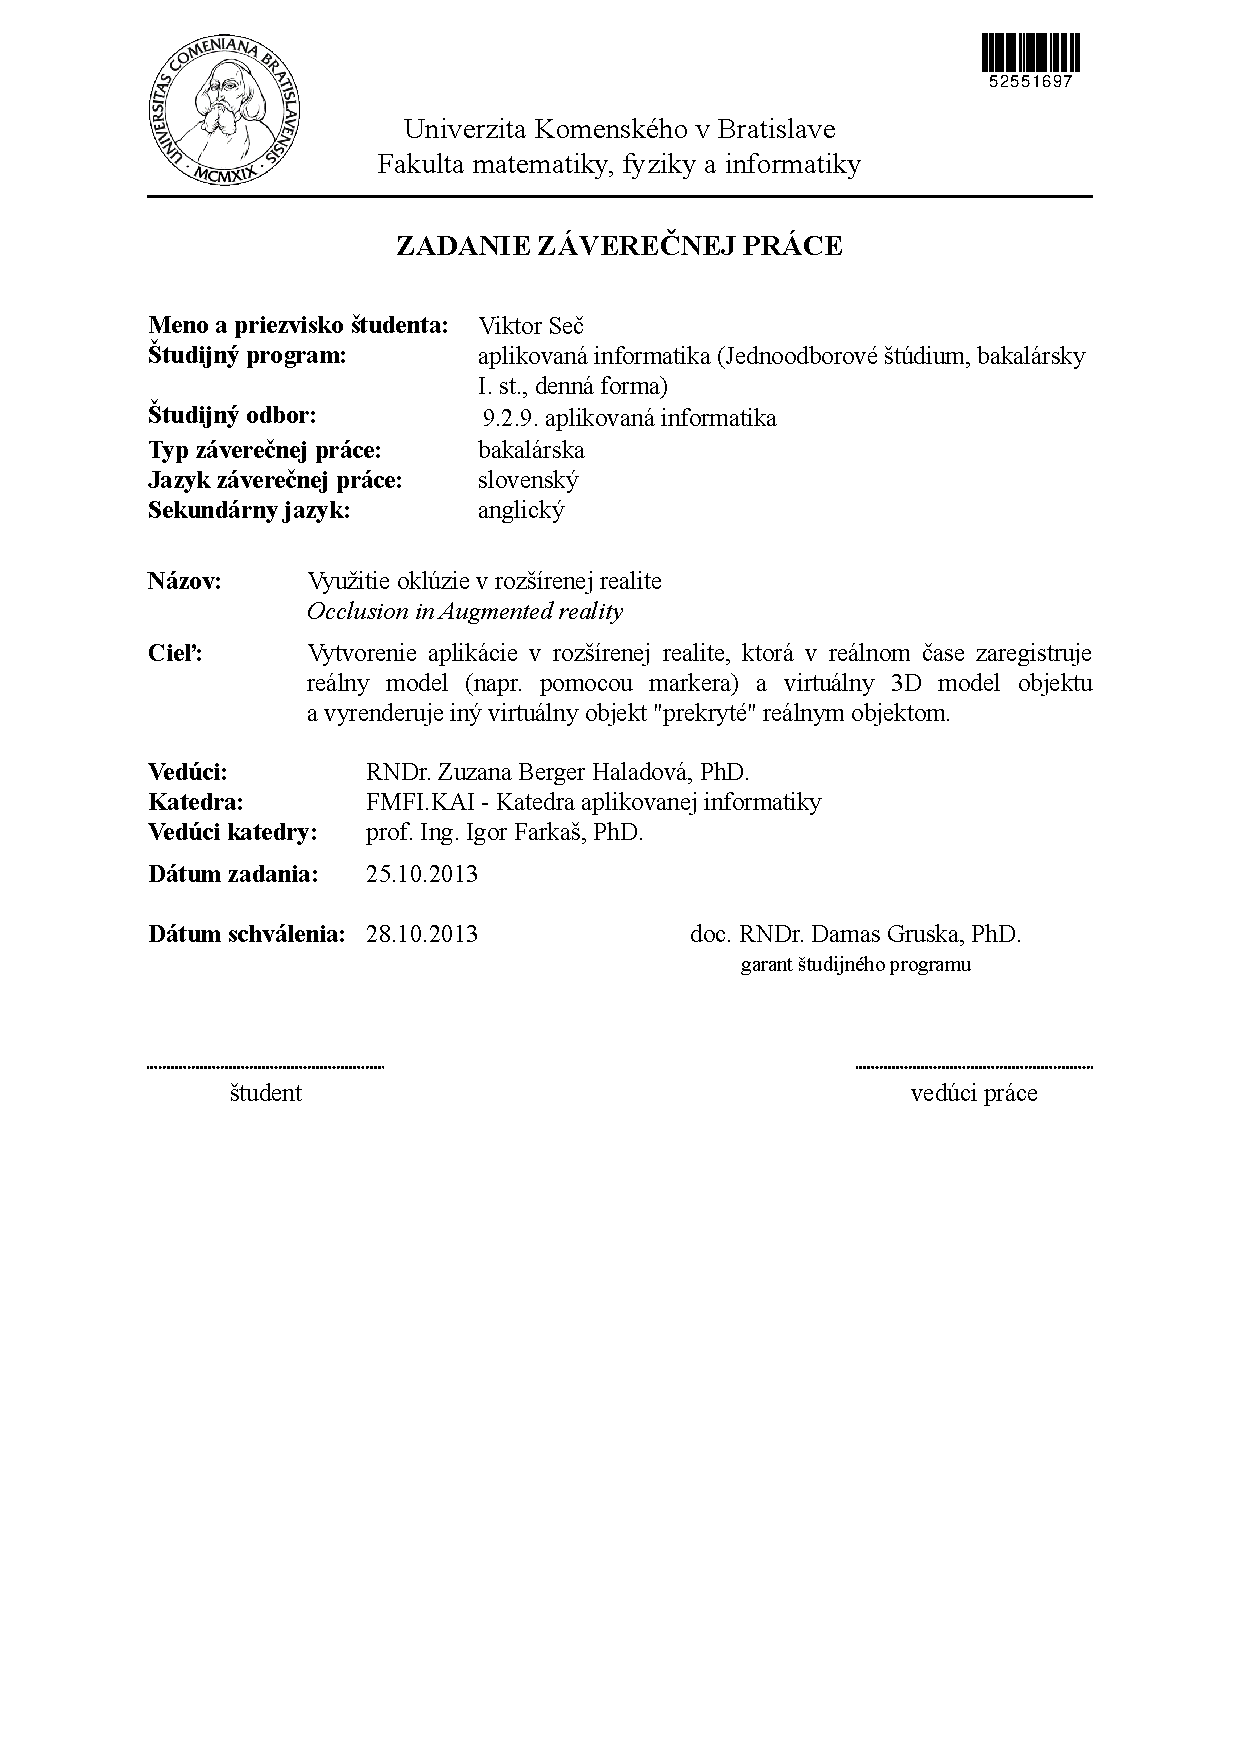
\includepdf[pages={1}]{zadanie.pdf}

%% prehlasenie
\iftrue
	\thispagestyle{empty}
	\vglue0pt

	\vfil

	\noindent\textbf{Čestné prehlásenie}

	\bigskip
	\begin{flushleft}
	Čestne vyhlasujem, že som bakalársku prácu vypracoval samostatne s použitím uvedenej odbornej literatúry.
	\end{flushleft}
	\bigskip

	\noindent Bratislava \today \hfil
	\begin{tabular}[t]{c}
	\hbox to 50mm {\dotfill} \\ \textit{\small Viktor Seč}
	\end{tabular} \qquad \linebreak

	\pagebreak
\fi



\thispagestyle{empty}
\chapter*{Poďakovanie}
Moja hlboká vďaka patrí RNDr. Zuzane Berger Haladovej, PhD. za jej cenné podnety, rady, nápady, neustálu prístupnosť a priateľskosť. Bez ktorejkoľvek z týchto vecí by táto práca nemohla byť takou, akou je.

Taktiež som vďačný organizácii FabLab Bratislava, ktorá mi sprístupnila 3D tlačiareň a poradila, ako s ňou narábať. Ďakujem tímu FTLab na našej fakulte za prístup k~3D skeneru SMISS. Ďalej ďakujem svojej kamarátke Katke, ktorá mi pomohla s korektúrou.

Záverom by som sa chcel poďakovať všetkým vývojárom, ktorí prispeli alebo prispievajú do slobodných softvérových knižníc ktoré som použil - ARToolKit, DevIL, GLEW, GLUT a OpenCV.
\pagebreak
\thispagestyle{empty}
\chapter*{Abstrakt}
Rozšírená realita je počítačovým rozšírením skutočného fyzického sveta o virtuálne objekty v reálnom čase. Táto práca pojednáva o jednotlivých používaných technikách a metódach na dosahovanie rozšírenej reality a o jej možných praktických využitiach. \par

Súčasťou riešenia práce je tvorba vlastnej aplikácie s rozšírenou realitou obohatenou o oklúziu s reálnymi objektmi. \par

\emph{Kľúčové slová: rozšírená realita, počítačové videnie, rozpoznávanie markerov, oklúzia}
\pagebreak
\thispagestyle{empty}
\chapter*{Abstract}
Augmented reality is a real time computer augmentation of the real physical world with virtual objects. This thesis describes the used techniques and methods in the field and also discusses the potential practical applications. \par

The thesis solution also includes development of custom application demostrating augmented reality. \par

\emph{Keywords: augmented reality, computer vision, marker registration, occlusion}
\pagebreak
\singlespacing
\thispagestyle{empty}
\tableofcontents
\thispagestyle{empty}
\onehalfspacing
\newpage

\pagenumbering{arabic}
\setcounter{page}{6}

\singlespacing
\thispagestyle{empty}
\listoffigures
\thispagestyle{empty}
\onehalfspacing
\newpage
\chapter*{Úvod}
\addcontentsline{toc}{chapter}{Úvod}
Rozšírená realita, teda počítačom obohatený pohľad na skutočný svet nachádza čoraz väčšie uplatnenie v zábave, medicíne, armáde, reklame a mnohých ďalších oblastiach ľudskej činnosti, najmä preto, že sa rozširujú hardvérové možnosti. To, na čo bolo kedysi treba drahé laboratórne vybavenie, ako výkonné počítače, profesionálne kamery a senzory, dnes dokáže takmer každý moderný mobilný telefón s kamerou. Rozšírená realita otvára nové možnosti interakcie medzi virtuálnym a fyzickým svetom, čo môže byť v budúcnosti veľmi zaujímavé.

O tejto téme je počuť čoraz viac a stojí za to sa ňou zaoberať, nakoľko jej aplikácie môžu byť veľmi užitočné, ako ukážeme neskôr. V práci rozoberáme jednotlivé možnosti aplikácii tejto technológie aj s konkrétnymi príkladmi.

V jadre práce pojednávame o niektorých metódach registrácie obrazu, používaných na vytvorenie rozšírenej reality a popisujeme krok za krokom ako sme vytvorili demo aplikáciu rozšírenú o oklúziu s reálnymi objektmi. Popisujeme načítanie modelov, registráciu scény, niekoľko spôsobov získania modelu oklúdera, kalibráciu kamery a samotné vykresľovanie oklúzie. Na konci kapitoly prezentujeme výsledky demo aplikácie.

Práca je ukončená krátkym pojednaním o perspektíve budúceho využitia tejto technológie a o tom, čo bude potrebné pre to, aby sa používanie rozšírenej reality
rozšírilo.

\chapter{Prehľad problematiky}

V tejto kapitole vysvetlíme, čo je rozšírená realita a ako bola definovaná. Popíšeme na~čo všeobecne slúži a akými spôsobmi sa používa. Popíšeme kedy nastáva oklúzia a definujeme oklúder.

\section{Definícia rozšírenej reality}

Rozšírená realita (po anglicky \emph{augmented reality}, skrátene \emph{AR}) je počítačom rozšírený pohľad na reálny svet. Je to variácia virtuálnej reality, v ktorej používateľ nevníma svet okolo seba a je prenesený do sveta virtuálneho. Tento virtuálny svet je úplne umelý a nezávislý. Oproti tomu, pri rozšírenej realite používateľ naďalej vníma skutočný svet okolo seba doplnený o virtuálne objekty \cite{Azuma97}. Ronald T. Azuma definuje rozšírenú realitu tromi pravidlami \cite{Azuma97}.

\begin{enumerate}
\item Rozšírená realita musí kombinovať reálne a virtuálne objekty.
\item Aplikácia musí prebiehať v reálnom čase a nejakým spôsobom reagovať na zmeny v prostredí, teda byť interaktívna.
\item Rozšírená realita musí byť registrovaná v trojdimenzionálnom priestore. To znamená, že musí korektne registrovať pohľad kamery s virtuálnym svetom a správne identifikovať, na ktoré pozície je potrebné vykresliť (po anglicky \emph{render}) virtuálne objekty.
\end{enumerate}

Cieľom rozšírenej reality môže byť v jednoduchšom prípade prezentovať používateľovi nejaké informácie (napríklad informácie o určitých skutočných objektoch, ako je ich vzdialenosť, poloha, identifikácia a podobne), alebo vykreslovať neskutočné objekty tak, aby vyzerali ako skutočné a patriace do okolitého prostredia. V druhom prípade je potrebné, aby boli tieto objekty trojdimenzionálne a vykresľovali sa správne v súlade s perspektívou a skutočnými objektami (napríklad prekrývali objekty za nimi, ale boli prekryté objektmi pred nimi) \cite{Azuma01}. V prvom prípade je však podľa Azumovej definície stále potrebné, aby sa dané informácie vykreslovali vo výstupe na správne miesta, závisiace od vstupu kamery, alebo iných senzorov. Príklady oboch sú uvedené v nasledujúcej kapitole.

Rozšírená realita sa, rovnako ako virtuálna realita, nemusí nutne týkať iba vizuálneho obrazu. Teoreticky by mohla ovplyvňovať každý druh senzorického vnímania. Je to však obtiažna úloha, pretože na rozdiel od virtuálnej reality, v
ktorej stačí tieto umelé zmyslové podnety len generovať, rozšírená realita musí upravovať skutočný svet. To znamená, že okrem dopĺňania virtuálnych objektov občas potrebuje retušovať skutočné objekty, aby zanikli. Na to, aby sa to dalo dosiahnuť je potrebné vedieť zablokovať určitú časť pôvodného vnemu \cite{Bimber05}.

V prípade zraku je potrebné prekresliť skutočný objekt pozadím, ktoré sa nachádza za ním. Pri sluchu je filtrovanie jednotlivých zvukových stôp zo zmixovaného vstupu a navyše v reálnom čase (napríklad odfiltrovanie hlasu niektorej osoby v miestnosti) obtiažnejším problémom.

Rozšírená realita sa z praktických dôvodov obvykle zameriava na obraz. Týmto aspektom sa zaoberá aj táto práca.

\section{Účel}

Dôvodov pre vývoj rozšírenej reality je niekoľko. Pre používateľa môže byť rozšírená realita jedným z najjednoduchších spôsobov ako získavať určité druhy
informácií. Toto môže zefektívňovať a zjednodušovať jeho skutočnú prácu. Obzvlášť prakticky vyzerajú napríklad koncepty, pri ktorých má používateľ špeciálne okuliare, ktoré mu zobrazujú požadované dáta zo senzorov a databáz priamo na sklá a používateľovi ostávajú voľné ruky na prácu.

Dobrým príkladom je napríklad aplikácia firmy Boeing, vyvinutá pre mechanikov servisujúcich lietadlá. Keď mechanik odstráni niektorý z krycích panelov na lietadle, môže namieriť kameru tabletu na zväzky káblov a rozvodov, ktoré sa pod ním nachádzajú. Softvér v reálnom čase na obrazovku dopĺňa údaje o tom, ktorý kábel, alebo trubica kam vedie a na čo slúži. Šetrí sa tak množstvo času oproti vyhľadávaniu v~hrubých manuáloch.

Rozšírená realita má samozrejme taktiež široké spektrum využitia v~zábave alebo marketingu.

\section{Zariadenia}

Rozšírená realita môže byť prezentovaná používateľovi buď priamo (napríklad vykreslovaním na priehľadný displej, cez ktorý je priamo vidno okolité prostredie), alebo nepriamo, čiže vykreslovaním do záznamu z videokamery, ktorý je vzápätí po rozšírení prezentovaný používateľovi na nepriehľadný displej.

\begin{figure}[h]
 \centering
 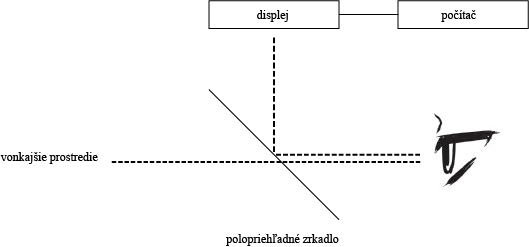
\includegraphics[scale=0.6]{pictures/schema-hmd}
 \caption{Schéma priamej rozšírenej reality}
 \label{prama-realita}
 \end{figure}

V prípade priamej optickej rozšírenej reality za použitia priehľadného displeja sa obvykle používa nejaký typ okuliarov, alebo helmy. Tieto okuliare obsahujú šikmú poloreflexnú plochu, cez ktorú je priamo vidno, ale taktiež odráža obraz z malého displeja umiestneného nad ňou, alebo pod ňou \cite{Bimber05}. Keď sa cez ne používateľ pozrie, obrazy sa mu skombinujú (znázornené na obrázku \ref{prama-realita}).

\begin{figure}[h]
 \centering
 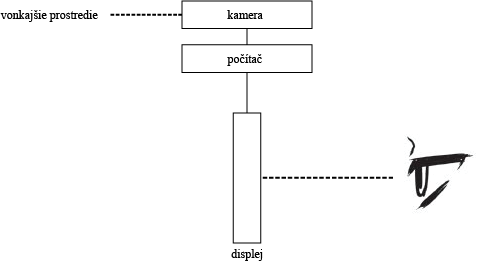
\includegraphics[scale=0.6]{pictures/schema-hmd-2}
 \caption{Schéma sprostredkovanej rozšírenej reality}
 \label{nepriama-realita}
 \end{figure}

Pre videom sprostredkovanú rozšírenú realitu sa používajú ľubovoľné zariadenia s~obrazovkami, ako sú telefóny, tablety, či počítače. Ani v tomto prípade však nie je vylúčené použitie špeciálnej helmy. Takéto helmy sa označujú ako HMD z anglického \emph{head-mounted display}. Podľa vysvetleného použitia sa delia na \emph{optical see through} (priame) a \emph{video see through} (sprostredkované). V demo aplikácií, ktorá bola vyvinutá ako súčasť tejto práce, ukazujeme sprostredkovanú rozšírenú realitu pomocou počítača, ku ktorému je pripojená kamera (znázornené na obrázku \ref{nepriama-realita}).

\section{Definícia oklúzie}

Oklúzia (po anglicky \emph{occlusion culling}), je proces počas ktorého algoritmus rozhoduje, ktoré objekty alebo prípadne časti objektov sú na scéne viditeľné. Pokiaľ je nejaký objekt sčasti alebo kompletne skrytý za iným objektom, znamená to, že je okludovaný a teda sčasti alebo vôbec nie je viditeľný (ilustruje obrázok \ref{sonofman}). Objekt, ktorý ho zakrýva sa nazýva oklúderom (po anglicky \emph{occluder}).

Oklúzia sa obvykle používa ako optimalizačná metóda (nie je potrebné vykresľovať pixely, ktoré budú napokon prekryté), v rozšírenej realite sa dá využiť tak, aby ilúzia pôsobila reálnejšie.

\begin{figure}[h]
 \centering
 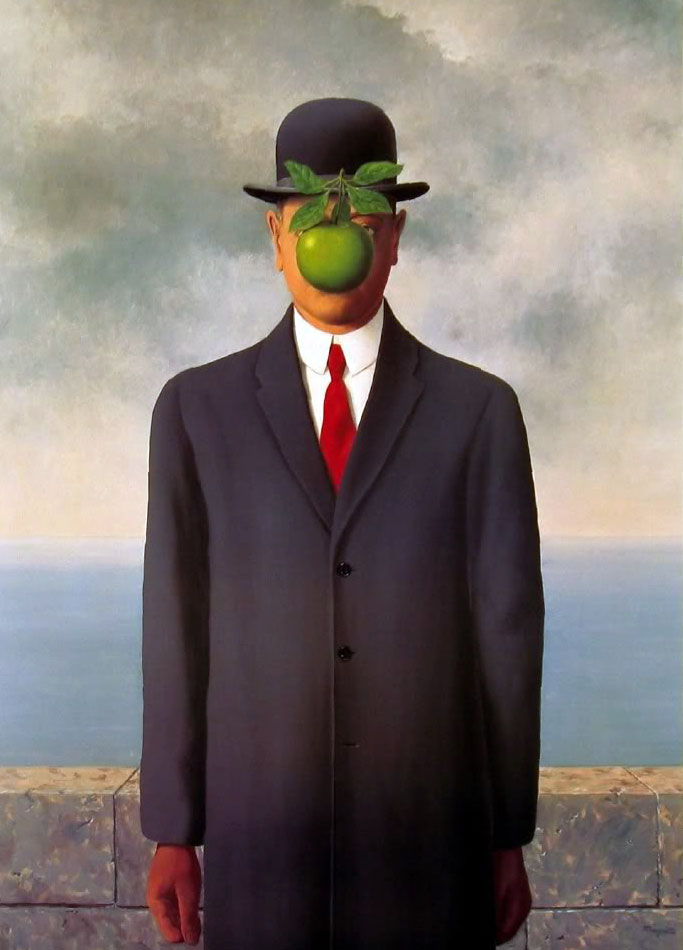
\includegraphics[scale=0.3]{pictures/sonofman.jpg}
 \caption[Na maľbe je mužova tvár čiastočne zakrytá jablkom. V 3D priestore by bolo jablko oklúderom.]{Na maľbe je mužova tvár čiastočne zakrytá jablkom\footnotemark. V 3D priestore by bolo jablko oklúderom.}
 \label{sonofman}
\end{figure}
\footnotetext{Obraz \emph{The Son of Man} namaľoval belgický umelec René Magritte.}
\chapter{Aplikácie}

Rozšírená realita má množstvo využití od zábavy až po záchranu životov. Nižšie sú vybrané niektoré z nich.

\section{Medicínske aplikácie}

Rozšírená realita by mohla mať bohaté využitie na poli medicíny. Lekárom by sa pomocou nej mohli vytvárať detailné vizualizácie vnútorných orgánov, nádorov a podobne a zobrazovať sa im prekryte priamo cez telo pacienta. Na získanie údajov by sa mohlo použiť ľubovoľné diagnostické zariadenie, ktoré produkuje 3D dáta o pacientovi. Napríklad vyšetrenie magnetickou rezonanciou, alebo ultrazvukom. Tieto vizualizácie by mohli byť obzvlášť cenné pri minimálne invazívnych zákrokoch, kedy vidí chirurg vnútro tela pacienta horšie, ako pri bežnej operácii \cite{Azuma97}.

Vedci z Mníchovského Institut für Informatik vyvinuli trenažér pre gynekológov na~nácvik pôrodov, ktorý využíva rozšírenú realitu. Pôvodný simulátor, ktorý vypisoval fiziologické dáta ako sú krvný tlak, tep, úroveň bolesti, či údaje o prívode kyslíka na monitor pristavený pri nemocničnej posteli, prestavali tak, aby sa všetky potrebné údaje vypisovali na okuliare špeciálnej helmy. Okrem vypisovania týchto jednoduchých dát sa však na okuliare dokresluje aj polopriehľadný virtuálny model dieťaťa uloženého v maternici. Na to, aby to bolo možné je potrebné registrovať vzájomnú polohu hlavy používateľa a simulátoru.


Podľa autorov hrá toto dôležitú rolu pri zvyšovaní efektivity tréningu, nakoľko sa lekár môže plne koncentrovať na simulovaný vaginálny pôrod namiesto sledovania počítačových monitorov \cite{Sielhorst04}.

V roku 2004 bol v Kalifornii vykonaný prvý úspešný chirurgický zákrok prevedený za asistencie rozšírenej reality. Štyridsaťpäťročný pacient podstúpil laparoskopickú adrenalektómiu (odobranie nadobličky). Chirurgovi sa pri operácií na monitor zobrazovala 3D rekonštrukcia nadobličiek a iných okolitých orgánov vsadená na správne miesto do pohľadu z kamery. Toto pozíciovanie sa vypočítavalo na základe siedmich markerov nalepených na koži pacienta \cite{Marescaux04}.

\section{Požiarnici}

Patrick Jackson, požiarnik zo Severnej Karolíny vyvíja požiarnicku aplikáciu pre Google Glass. Do okuliarov sa mu premietajú údaje od operátora tiesňovej linky, mapy a ukazovateľ k najbližšiemu hydrantu. V budúcnosti má zobrazovať napríklad aj plány budov, alebo schémy rozrezávania vrakov
jednotlivých modelov áut \cite{Google14-a}. Na zobrazovanie mapy okolia sa využívajú údaje z GPS a na navigovanie k hydrantu aj presné natočenie hlavy. Táto aplikácia je ukážkovým príkladom, ako by mohla rozšírená realita v kritických situáciach zachraňovať životy.

Podobný softvér (s vlastným hardvérom) vyvíja tím na Technickej univerzite vo~Viedni. Požiarnikovi ukazujú v okuliaroch obraz z termálnej kamery registrovaný s~3D modelom štruktúry budovy, ktorý je rekonštruovaný v reálnom čase (obrázok \ref{poziarnici}). Vďaka tomu vie ako vyzerá jeho okolie aj v prípade hustého dymu \cite{Schonauer13}.

\begin{figure}[h]
 \centering
 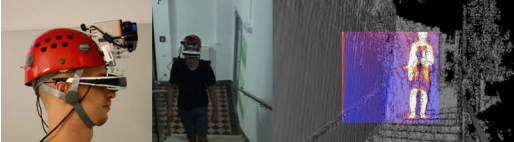
\includegraphics[max width=\textwidth]{pictures/wien-firefighters.png}
 \caption{Projekt má požiarnikom zabezpečiť životne dôležité informácie v podmienkach slabej viditeľnosti \cite{Schonauer13}}
 \label{poziarnici}
 \end{figure}

\section{Preklady}

Na University of California vytvorili mobilnú aplikáciu, ktorá cez rozšírenú realitu prekladá text. Používateľ jednoducho namieri telefón na nápis, ktorý chce preložiť, a~aplikácia text v obraze z kamery zdeteguje pomocou optického rozoznávania znakov. Softvér vzápätí text preloží a vykreslí na obrazovku telefónu priamo do videa z kamery. Pri tomto vložení dbá nielen na to, aby preložený text umiestnil na správne miesto a~v~správnej farbe a veľkosti, ale aj aby vyretušoval pôvodný text, ktorý by bol umiestnený pod tým preloženým \cite{Fragoso11}. Ukážka aplikácie je na obrázku \ref{translatar}.

\begin{figure}[h]
 \centering
 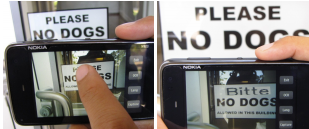
\includegraphics[max width=\textwidth]{pictures/translatar.png}
 \caption{Ukážka aplikácie TranslatAR \cite{Fragoso11}}
 \label{translatar}
 \end{figure}

\section{Armádne aplikácie}

Vojenské operácie sa často vykonávajú v mestskom prostredí. Bojové zóny, v ktorých sa nachádzajú poschodové budovy sú veľmi komplikované a pre~úspech misie sú pre vojaka mimoriadne dôležité informácie o okolí. Keď vojak pozerá do mapy, ohrozuje sa, pretože dáva nižší pozor na svoje okolie.

Vedci z Naval Research Laboratory v USA vytvárajú helmu, ktorá bude vojakom sprostredkovávať najdôležitejšie informácie. Používateľ môže vidieť nad budovami napísané ich mená a plány interiérov, na zemi zas môže vidieť napísané názvy ulíc. Taktiež sa mu môžu zobrazovať ikony na presných lokáciach, kde boli nahlásení ostreľovači~\cite{Livingston02, Julier00}.

Inou aplikáciou rozšírenej reality na armádne účely je systém rozširujúci videnie pilota lietadla. Úlohy ako zameriavanie cieľa, dodávky zbraní a zásob na padákoch, či obyčajný let v nízkej výške vyžadujú, aby pilot presne rozoznával terén pod sebou. Senzory na stíhačke môžu sledovať oblasť, ktorú pilotovi v zornom poli zakrýva samotné lietadlo, alebo mu poskytovať dáta za podmienok slabej viditeľnosti. Všetky tieto dáta sa potom môžu premietať do pilotovej helmy, umožniť mu vidieť to, čo by inak nevidel a zvýrazniť dôležité body \cite{Livingston11}.

Prvé podobné primitívne systémy vznikli už pred Druhou svetovou vojnou. Spojeneckí piloti používali v niektorých lietadlách napríklad Mark II Gyro Sight, teda gyroskopický zameriavač. Toto zariadenie pilotovi ukazovalo na polopriehľadný displej, kam poletí strela na základe údajov z gyroskopu a meraču rýchlosti.

Rozšírená realita prenikla na poli letectva aj do civilnej sféry. Na obrázku \ref{boeing} je pilotná kabína Boeingu pri navádzaní na pristátie.
 
Podobné aplikácie by mohli mať význam aj pre vojenské a civilné pozemné dopravné prostriedky.

\begin{figure}[h]
 \centering
 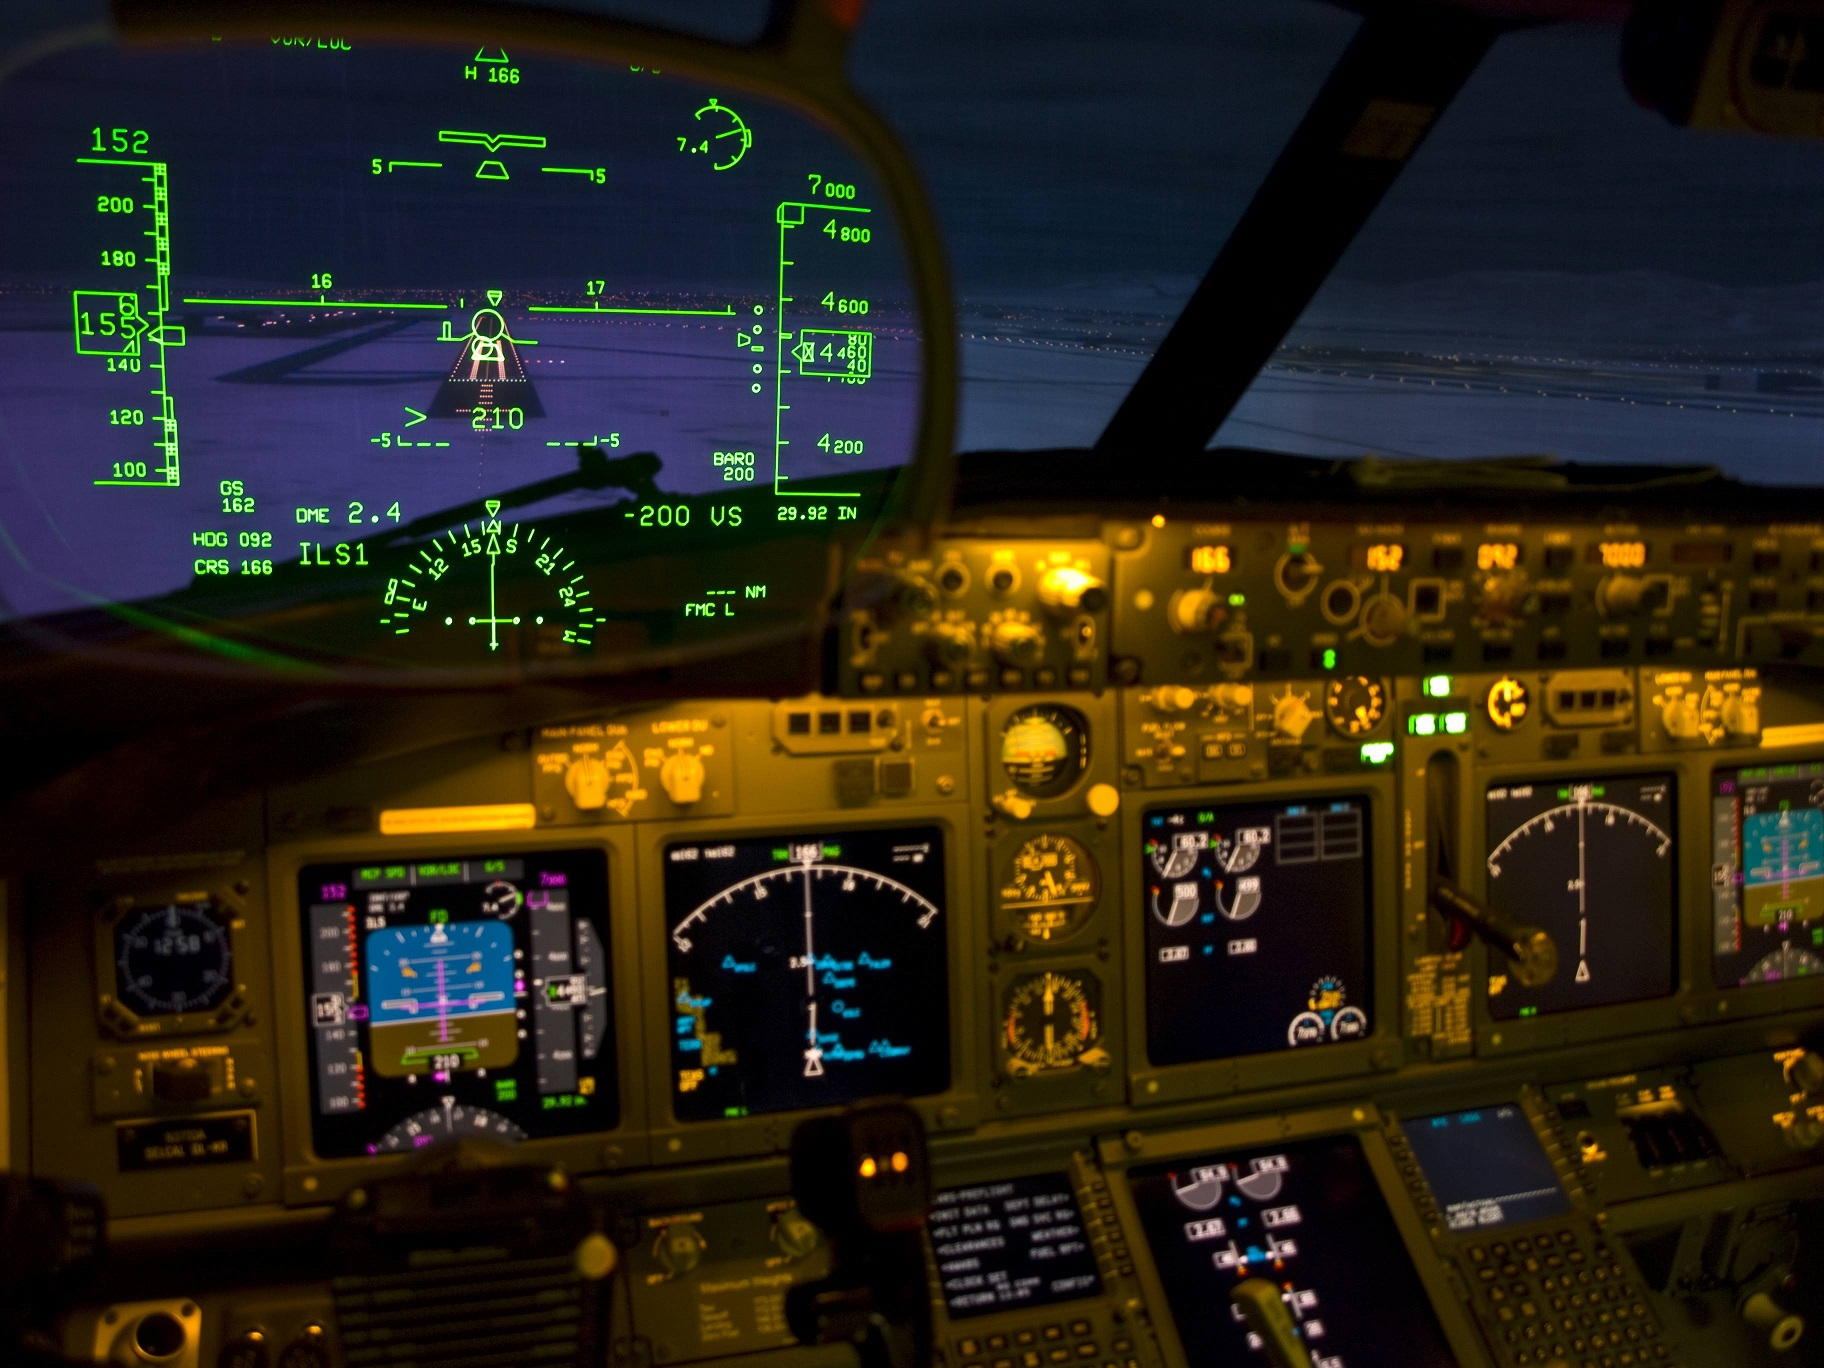
\includegraphics[max width=\textwidth]{pictures/kokpit.jpg}
 \caption{Rozšírená realita v kokpite lietadla Boeing 737-800; Autor: Barend Havenga \cite{Havenga}}
 \label{boeing}
\end{figure}

\section{Šport}

Pri športových televíznych prenosoch je používanie rozšírenej reality pomerne bežné. Prvý krát bol prenos rozšírený už počas Olympijských hier 1996 a napríklad firma Sportvision dodnes virtuálne rozširuje prenášané záznamy už od roku 1998.

Na hraciu plochu dokážu zobrazovať rôzne dočasné čiary a zóny, informácie o bodovom stave, logá, zástavy a podobne a to tak, že sú prekrývané skutočnými hráčmi, ktorí sú na nej. Podobnými spôsobmi rozširujú napríklad televízne prenosy z NHL, NFL, alebo NASCAR \cite{Sportvision, Ismert12}. Mimo Spojených štátov sú zrejme najznámejšími virtuálne zástavy dokreslované do plaveckých bazénov na Olympijských hrách, prípadne čiara, ktorá sa počas preteku posúva pozdĺž bazénu a označuje svetový, alebo Olympijský rekord.

\section{Konštrukcia}

Rozšírená realita by mohla pomôcť aj stavbárom, či statikom. V okuliaroch by im do~reálneho pohľadu mohli byť dokresľované napríklad stĺpy za stenami, presné polohy roxorových tyčí získané magnetickými senzormi, káble vedúce elektrinu v stenách, či~samotné označenia nosných stien \cite{Webster96}.

Iné využitie uľahčuje prácu mechanikom. Napríklad bola vyvinutá aplikácia, ktorá zobrazuje automechanikovi do helmy všetky súčiastky vo dverách auta. Výmena zámku, či motorčeku na otváranie okna je pri tomto modeli vozidla pomerne obtiažna, pretože automechanik musí strčiť ruky dnu do dverí a nevidí, čo robí. Do aplikácie boli nahrané modely všetkých súčiastok a tá ich premieta na
ich skutočné miesto \cite{Reiners98}.
\chapter{Metódy}

Pre dosiahnutie rozšírenej reality je potrebné rozoznať, na ktoré miesto v obraze sa má vykresliť daný virtuálny objekt. Tiež treba správne rozhodnúť, aký má byť tento objekt veľký a ako má byť natočený. Na toto rozhodnutie je treba poznať vzájomnú polohu virtuálneho objektu a kamery, respektíve očí používateľa.

Na riešenie problému sa obvykle používajú metódy počítačového videnia. Na ich aplikáciu je potrebné zariadenie s digitálnou kamerou, ktorej záznam softvér analyzuje.

Inou možnosťou je získať informáciu o polohe a smere zorného poľa pomocou iných senzorov. Tento prístup sa dnes používa, ale vymyká sa pôvodnej Azumovej definícii rozšírenej reality \cite{Azuma97} (pozri článok 1.1).

\section{Rozpoznávanie pomocou markerov}

Najjednoduchší spôsob, ako sa dá tento prístup implementovať, je za pomoci markerov. Markery sú obvykle jednoduché asymetrické čiernobiele značky, ktoré sa umiestnia do skutočného sveta tak, aby boli vždy v zábere kamery. Je potrebné zaznačiť, aká je presná poloha, na ktorú sa má vykresliť virtuálny objekt voči tomuto statickému markeru. Občas sa vykresluje priamo na marker, ale obvyklejšie je umiestniť marker len niekam do pozadia. Softvér s rozšírenou realitou potom hľadá vo videu tento marker a keď ho odhalí, tak nájde transformáciu, ktorá marker posunie, otočí a zoškáluje do veľkosti ako je vo videu. Touto transformáciou sa potom transformuje aj virtuálny model, ktorý sa vzápätí vykreslí buď späť do videa, alebo zvlášť na priehľadný displej.

Technológia má presnosť umiestňovania jednotlivých objektov závislú od kvality snímaného obrazu. Vyskytujú sa však chyby, kedy aplikácia pre zlú viditeľnosť nerozozná marker a nič nevykreslí, alebo rozozná za marker skutočný objekt, ktorý markerom nie je a vykreslí virtuálny objekt aj keď ho vykresliť nemá. Ďalšiou nevýhodou je samozrejme to, že v momente, keď sa stratí marker zo záberu, prestane sa vykreslovať aj k nemu prislúchajúci objekt. Tento problém sa dá riešiť buď inštalovaním siete markerov do pozadia, ktoré v sebe majú zakódované svoje súradnice, alebo sledovaním (\emph{trackovaním}) pohybu kamery\footnote{Dá sa namerať priamo z optického toku dát, pomocou informácií z gyroskopu, akcelerometra, magnetometra, alebo ich kombinácie.}. Softvéru potom stačí, aby bol v zábere kamery dobre viditeľný vždy aspoň jeden. Pokiaľ markery neznehodnotia scénu a vývojári potrebujú maximalizovať šance systému na správnu registráciu, môžu sa rozhodnúť použiť pole markerov (po anglicky \emph{marker field}), ktoré pokrýva kompletný povrch scény.

\subsection{Algoritmus rozpoznávania markerov}

Hľadanie markerov sa zvykne robiť nasledovným postupom, ktorý sa zvlášť aplikuje na~každý snímok z kamery. Snímok najprv prejde prahovaním, čo znamená, že sa zmení na binárny. Určí sa istý prah jasu a každý bod obrázku, ktorý má vyšší jas sa prefarbí na biely a všetky ostatné sa prefarbia na čierne. Výsledkom je binárny obraz. Ak sa prah nastaví správne malo by byť v tomto obraze jasne vidno aspoň jeden čiernobiely marker na jednofarebnom pozadí \cite{Kato99}.

Ako ďalší krok sa označia jednotlivé jednofarebné komponenty a~zdetegujú sa ich kontúry. Kontúry sa rozdelia na úsečky a softvér medzi nimi označí priesečníky. Tie, ktoré sú blízko pri sebe a súčet uhlov medzi nimi je blízky 180 stupňom sa odignorujú, pretože tvoria takmer rovnú čiaru a výrazne nemenia tvar objektu. Komponenty, ktoré nemajú štyri ostré vrcholy sa vyradia, pretože nemajú štvorcový tvar. Zvyšné komponenty ostanú kandidátmi na markery. Algoritmus ďalej nájde všetky možné homografie, ktoré zobrazia rohy štvorca na rohy týchto komponentov. Výsledkom sú rotačné matice, ktorými sa transformujú uložené obrázky markerov. Týchto markerov môže byť viac, napríklad ak chce program zobrazovať rôzne objekty na rôzne markery. Po tom, čo sa pre každý komponent vypočítajú cez všetky jeho matice všetky markery z pamäte, sa tieto výsledné obrázky prekryjú s originálnym snímkom a porovnajú \cite{ARToolKit-a}. Binárny obrázok s komponentmi už ďalej nie je potrebný. Pri porovnávaní originálneho snímku s pretransformovaným markerom sa použije niektorá z metód hodnotenia podobnosti. Napríklad sa pre každý pixel vypočíta hodnota rozdielu jasu a potom sa urobí suma všetkých týchto hodnôt. Čím je výsledná hodnota nižšia, tým sú si obrázky podobnejšie.

Pre každého kandidáta na marker sa vyberie ten obrázok, ktorý je mu najpodobnejší a zapamätá sa akou konkrétnou homografiou vznikol. Ak je podobnosť nižšia ako istá hranica, kandidát sa vymaže z výberu a považuje sa za chybu. Výsledkom je zoznam jednotlivých kandidátov, ich súradníc v rámci snímky, k nim prislúchajúce identifikácie markerov (ak sa v aplikácí používa viac markerov) a homografie, určujúce ako na ne niečo premietnuť.

V prípade, že je snahou umiestniť virtuálny objekt priamo na marker, môže sa na~jeho 3D model použiť daná homografia, čím sa správne umiestni, naškáluje a zrotuje, a~vykreslí buď do pôvodného snímku, alebo na priehľadný displej. Ak je marker posunutý, považuje sa za počiatok súradnicovej sústavy a virtuálny objekt sa adekvátne posunie.

Marker samozrejme nemusí byť čiernobiely ani štvorcový, v týchto prípadoch sa algoritmus príslušne upraví. Nakoľko vypočítavanie celého tohoto postupu pre každý snímok v reálnom čase môže byť náročné, často sa využívajú techniky sledovania pohybu. To znamená, že si program pamätá pre objekt jednotlivé polohy a homografie z predchádzajúcich snímkov a prednostne ich vyskúša. Taktiež môže pri plynulom pohybe predpovedať lokácie na nasledovných snímkoch.

Kroky tohoto algoritmu sú znázornené na obrázku \ref{artoolkit}.

\begin{figure}[h]
 \centering
 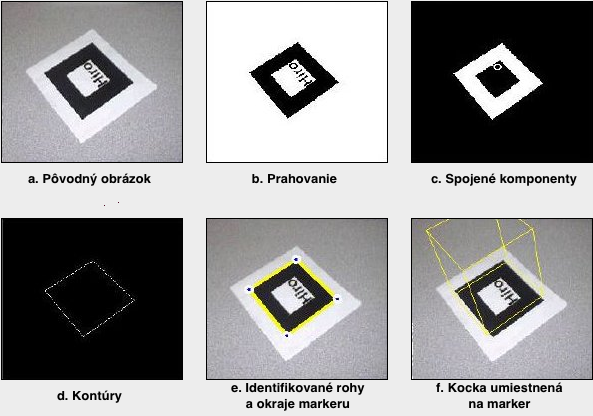
\includegraphics[max width=\textwidth]{pictures/artoolkit.png}
 \caption{Jednotlivé kroky aplikované pri rozpoznávaní markeru, tak ako sú uvedené v dokumentácií knižnice ARToolKit \cite{ARToolKit-a}}
 \label{artoolkit}
\end{figure}

Implementáciu tohoto algoritmu v knižnici ARToolKit využívame aj v demo aplikácii vytvorenej v rámci tejto práce.

\section{Rozpoznávanie na základe významných bodov}

V prípade, že nie je žiadúce použitie markeru, pretože nie je možné modifikovať prostredie, prípadne je potrebné, aby aplikácia fungovala aj v prostrediach, ktoré na tento účel neboli predpripravené, je potrebné túto úlohu riešiť zložitejšiou analýzou. Pri riešení týmto spôsobom musí byť známe ako vyzerá okolie, do ktorého je žiadané vykresliť virtuálny objekt. Toto okolie je potom potrebné rozoznávať v zábere kamery. Táto metóda sa obvykle používa na aplikácie, ktoré napríklad dopisujú v galérií údaje k~obrazom a podobne. V tomto prípade slúži obraz ako špeciálny marker.

\subsection{Rozpoznávanie algoritmom SIFT}
\emph{Scale-invariant feature transform}, alebo SIFT je algoritmus na rozpoznávanie a popisovanie významných bodov vyvinutý Davidom Lowe. Idea je, že objekt, ktorý chceme rozoznávať obsahuje významné body, ktoré sa dajú popísať. Výsledkom je deskriptor, s pomocou ktorého sa dá tento objekt
lokalizovať na iných obrázkoch.

Algoritmus generuje z obrazu objektu množstvo vektorov významných bodov. Tieto vektory sú invariantné na rotáciu a škálovanie obrazu. Významné body obvykle ležia na rohoch, hranách a iných kontrastných miestach, vďaka čomu sú dobre viditeľné aj za~zhoršených podmienok. Pri detekcii sa potom vyhľadáva v tejto databáze významných bodov \cite{Lowe99, Volosin11}.

Jednou z výhod algoritmu SIFT je, že dokáže rozpoznávať aj objekty, ktoré sú čiastočne zakryté. Jedným z následníkov SIFT je napríklad SURF (celý názov \emph{Speeded Up Robust Features}), ktorý je približne osem krát rýchlejší. SURF je
patentovaný Herbertom Bayom \cite{Bay06}. Ďalšími algoritmami na rozpoznávanie významných bodov sú BRIEF \cite{Calonder10} (\emph{Binary Robust Independent Elementary Features}), ktorý má podobné alebo lepšie výsledky ako SURF, BRISK (\emph{Binary Robust Invariant Scalable
Keypoints}) \cite{Leutenegger11}, FREAK (\emph{Fast Retina Keypoint}) \cite{Alahi12}, SUSSAN \cite{Smith97}, FAST \cite{Tuzel06} a DAISY \cite{Tola10}.

\section{Rozpoznávanie na základe GPS}

V prípade, že sú známe presné polohy virtuálnych objektov a nie je známe ako vyzerá okolie, do ktorého sa majú tieto objekty vykresliť, ako napríklad pri aplikáciach, čo do reálneho sveta dokreslujú mapu okolia, názvy firiem a podobne, problém sa rieši pomocou GPS. Tieto aplikácie majú databázu, v ktorej majú pri všetkých údajoch obsiahnuté aj súradnice GPS. Používateľ potom potrebuje zariadenie s GPS a digitálnym kompasom, ktoré na základe dát z GPS a kompasu vypočíta, na ktorý objekt v databáze je namierená kamera, alebo hlava používateľa, kde by sa tento objekt mal nachádzať v zábere a pod akým uhľom a v akej veľkosti ho má byť vidno \cite{Bimber05}.

Aby aplikácia spĺňala Azumovu definíciu rozšírenej reality, je túto metódu potrebné skombinovať s metódami rozpoznávania obrazu. V praxi však existujú aj aplikácie, ktoré sa spoliehajú čisto na dáta z GPS a v prípade použitia zariadenia s priehľadným displejom, kameru ignorujú, pretože žiadnu analýzu obrazu nevykonávajú. Táto metóda je všeobecne menej presná ako metódy rozpoznávania obrazu, pretože používané senzory obvykle nie sú také presné a virtuálne objekty sa teda nemusia vykresliť presne na to správne miesto a môžu byť posunuté. Malou výhodou techniky je, že by sa pri~jej používaní nemali vyskytovať chyby, kedy nevykreslíme objekt (napríklad ako pri nerozoznanom markeri), prípadne chyby, pri ktorých sa vykreslí objekt na miesto, na ktoré sa žiaden objekt vykresliť nemá.

\section{Prehľad softvérových knižníc }

Existuje niekoľko softvérových knižníc uľahčujúcich implementáciu aplikácií vytvárajúcich rozšírenú realitu.

Jednou z prvých takýchto knižníc je ARToolKit vyvinutý Hirokazu Katom v roku 1999 pre jazyky C a C++. Táto knižnica deteguje markery a prepočítava pod~akým uhlom ich používateľ vidí. Vývojárom ďalej poskytuje súradnicový systém, ktorý do tohoto priestoru transformuje. ARToolKit je k dispozícií zadarmo pod licenciou GNU/GPL \cite{ARToolKit-b}. Z tejto knižnice vychádza množstvo ďalších nasledovníkov a dodnes sa používa. Využívame ju za účelom registrácie objektov v aplikácii s~rozšírenou realitou, ktorá je súčasťou tejto práce.

ARToolkitPlus bol otvorený tracker, ktorý vychádzal z ARToolKitu. Jeho vývoj sa zastavil v roku 2007 a bol nahradený Studierstube trackerom, ktorý už však nie je verejne prístupný \cite{Wagner07}.

Studierstube je framework vyvinutý na \emph{Graz University of Technology}. Na trackovanie sa odporúča použiť OpenTracker od rovnakých autorov. Vývoj bol ukončený v~roku 2008 \cite{Studierstube-a, Studierstube-b}.

ArUco je minimalistická knižnica pre C++. Rozpoznáva markery, alebo polia markerov a je veľmi rýchla vďaka tomu, že sa opiera o OpenCV \cite{ArUco}.

Vuforia je proprietárnou knižnicou, ktorá dokáže rozpoznávať obrázky a jednoduché 3D objekty. Dá sa používať v C++, Jave a Objective-C, vďaka čomu je obľúbená na~mobilných platformách iOS a Android \cite{Vuforia}.
\chapter{Implementácia}

V rámci riešenia práce sme navrhli aplikáciu na demonštráciu rozšírenej reality obohatenú o oklúziu fyzických objektov.

V tejto kapitole popisujeme proces vývoja demo aplikácie od začiatku po finálnu verziu. Pre takúto demonštráciu je potrebné vyriešiť niekoľko problémov. Získať, alebo vyrobiť samotný oklúder a jeho digitálnu 3D reprezentáciu. Je potrebné vymodelovať objekty, ktoré chceme vykreslovať a naimportovať ich do grafickej knižnice. Tiež potrebujeme nejakým spôsobom registrovať scénu, do ktorej chceme objekty vykresľovať. Potrebujeme nakalibrovať kameru, aby bola ilúzia čo najpresnejšia. Na záver potrebujeme vyriešiť, ako implementovať samotnú oklúziu.

Táto kapitola opisuje všetky kroky schémy znázornenej na obrázku \ref{schema}.

\begin{figure}[h]
 \centering
 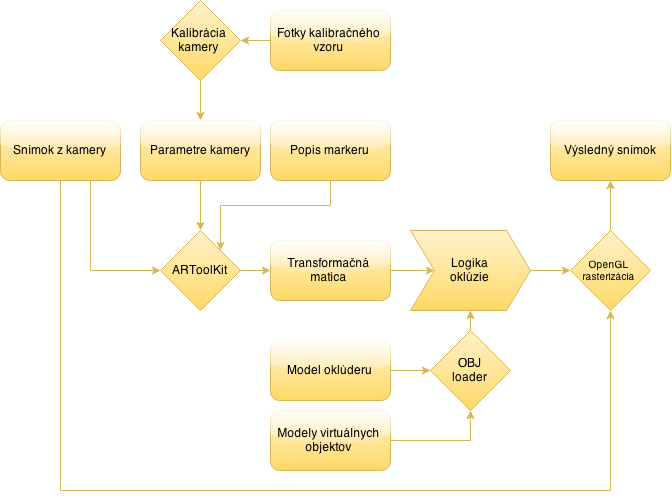
\includegraphics[max width=\textwidth]{pictures/schema.png}
 \caption{Podrobná schéma demo aplikácie}
 \label{schema}
 \end{figure}

\section{Zjednodušená demonštrácia}
\label{section-prototyp}

Na obrázku je snímok obrazovky prvého funkčného prototypu našej demo aplikácie. Aplikácia registruje scénu pomocou markeru a dokresľuje na ňu virtuálnu kocku okludovanú fyzickou kockou. Na obrázku \ref{prototyp} sa nachádza snímok obrazovky tohto skorého prototypu. Kroky tohto procesu sú chronologicky popísané v nasledujúcich sekciách.

\begin{figure}[h]
 \centering
 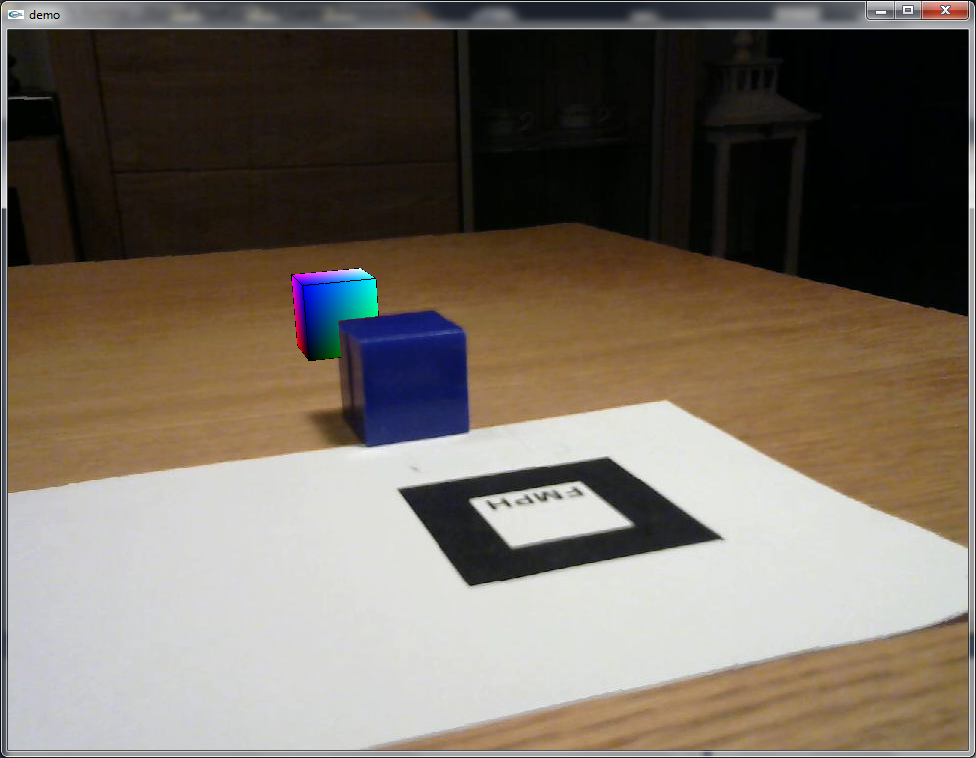
\includegraphics[max width=\textwidth]{pictures/screenshot-cubes.png}
 \caption{Jednoduchá ukážka oklúzie s kockami v našej aplikácii}
 \label{prototyp}
 \end{figure}

\section{3D modely}

Aby bolo možné vykresľovať 3D objekty na obrazovku, je potrebné ich reprezentovať v pamäti. Počas behu programu sa o to stará grafická knižnica, ale najjednoduchší spôsob ako do nej dáta naimportovať je uložiť ich do súboru.

Pre prácu s 3D modelmi existujú štandardizované formáty. Koncom deväťdesiatych rokov bol obľúbený formát VRML\footnote{Číta sa \emph{vermal}.}, ktorý je aj natívne podporovaný v ARToolkite, neskôr ho nahradil následník X3D \cite{Web3D}. Medzi dnes používanejšie formáty patrí napríklad COLLADA vyvíjaná združením Khronos Group \cite{Collada}, jej výhodou je vysoká kompatibilita s väčšinou nástrojov na modelovanie aj hernými enginmi. Iným obľúbeným formátom je STL (\emph{stereolithography}) používaný najmä na inžinierske účely ako je automatické projektovanie (po anglicky \emph{computer-aided design}, alebo \emph{CAD}) a~3D tlač. Výhodou je možnosť ukladania do textových aj binárnych súborov.

Zrejme najpoužívanejším 3D formátom je dnes Wavefront OBJ vyvinutý už neexistujúcou firmou Wavefront Technologies. OBJ je jednoduchý otvorený formát, ktorý sme sa rozhodli použiť.

\subsection{Formát Wavefront OBJ}

OBJ sme si vybrali, pretože sa jednoducho spracováva (\emph{parsuje}) a zároveň je všeobecne používaný a kompatibilný.

Formát vie zaznamenávať vrcholy (\emph{vertexy}), ich normály, textúrne súradnice a steny. Steny sú reprezentované n-uholníkmi danými zoznamami už definovaných vrcholov. Tieto vrcholy sú v zoznamoch uvedené v poradí v smere hodinových ručičiek \cite{Wavefront}.

Na ukážke \ref{dodecahedron} je zapísaný jednoduchý dvanásťsten vo formáte OBJ.

\lstset{ %
  backgroundcolor=\color{myyellow},
  breakatwhitespace=false,         % sets if automatic breaks should only happen at whitespace
  breaklines=true,                 % sets automatic line breaking
  commentstyle=\color{dkgreen},    % comment style
  keepspaces=true,                 % keeps spaces in text, useful for keeping indentation of code (possibly needs columns=flexible)
  keywordstyle=\color{blue},       % keyword style
  language=Python,                 % the language of the code
  otherkeywords={v, f},            % if you want to add more keywords to the set
  numbers=left,                    % where to put the line-numbers; possible values are (none, left, right)
  numbersep=5pt,                   % how far the line-numbers are from the code
  numberstyle=\tiny\color{gray}, % the style that is used for the line-numbers
  stepnumber=2,                    % the step between two line-numbers. If it's 1, each line will be numbered
  stringstyle=\color{mauve},     % string literal style
  tabsize=2,                       % sets default tabsize to 2 spaces
  title={dodecahedron.obj},                   % show the filename of files included with \lstinputlisting; also try caption instead of title
  caption={Dvanásťsten uložený vo formáte OBJ}
}

\begin{lstlisting}[label={dodecahedron}]
# Dodecahedron
v  -0.57735  -0.57735  0.57735
v  0.934172  0.356822  0
v  0.934172  -0.356822  0
v  -0.934172  0.356822  0
v  -0.934172  -0.356822  0
v  0  0.934172  0.356822
v  0  0.934172  -0.356822
v  0.356822  0  -0.934172
v  -0.356822  0  -0.934172
v  0  -0.934172  -0.356822
v  0  -0.934172  0.356822
v  0.356822  0  0.934172
v  -0.356822  0  0.934172
v  0.57735  0.57735  -0.57735
v  0.57735  0.57735  0.57735
v  -0.57735  0.57735  -0.57735
v  -0.57735  0.57735  0.57735
v  0.57735  -0.57735  -0.57735
v  0.57735  -0.57735  0.57735
v  -0.57735  -0.57735  -0.57735
f  19  3  2
f  12  19  2
f  15  12  2
f  8  14  2
f  18  8  2
f  3  18  2
f  20  5  4
f  9  20  4
f  16  9  4
f  13  17  4
f  1  13  4
f  5  1  4
f  7  16  4
f  6  7  4
f  17  6  4
f  6  15  2
f  7  6  2
f  14  7  2
f  10  18  3
f  11  10  3
f  19  11  3
f  11  1  5
f  10  11  5
f  20  10  5
f  20  9  8
f  10  20  8
f  18  10  8
f  9  16  7
f  8  9  7
f  14  8  7
f  12  15  6
f  13  12  6
f  17  13  6
f  13  1  11
f  12  13  11
f  19  12  11
\end{lstlisting}

Riadky začínajúce mriežkou slúžia na komentáre. Riadok začínajúci znakom \emph{v}~reprezentuje vrchol a obsahuje tri súradnice\footnote{Môže obsahovať štyri homogénne súradnice}. Riadky začínajúce znakmi \emph{vt} obsahujú textúrne súradnice zaznačené dvomi, či tromi číslami. Riadky začínajúce sa na~\emph{vn}~obsahujú normály vrcholov uložené tromi číslami.

Steny sú uložené na riadkoch začínajúcich znakom \emph{f}, po ktorom nasleduje zoznam vrcholov. Tieto vrcholy sú označené číslami, ktoré sa odvolávajú na poradie, v ktorom boli predtým definované. Steny môžu v svojich vrcholoch uchovávať aj textúrne súradnice, prípadne normály vrcholov. Tieto ďalšie informácie sa značia tak, že za poradové číslo vrcholu napíšeme lomku a pridáme poradové číslo predtým definovaných textúrnych súradníc. Za ďalšiu lomku môžeme zaznačiť poradové číslo normály. Pokiaľ je potrebné zaznamenať iba vrcholy a ich normály, vložia sa medzi ne dve lomky~\cite{Wavefront}.

Aby sme si ušetrili starosti pri spracovávaní a vykresľovaní modelu, rozhodli sme sa ho reprezentovať trojuholníkovou sieťou (po anglicky \emph{triangulated geometry}). To znamená, že každá stena je rozložená na steny ktoré majú len tri vrcholy. To má tú výhodu, že tieto trojuholníky sa dajú neskôr jednoducho vykreslovať pomocou OpenGL.

Na trianguláciu modelov sme použili otvorený modelovací nástroj Blender, ktorý dokáže exportovať modely do formátu OBJ v tejto podobe. OBJ príklad z ukážky \ref{dodecahedron} bol vytvorený týmto spôsobom.

Takto pripravený súbor načítame, spracujeme a vrcholy, normály a steny si uložíme do polí, z ktorých ich cez OpenGL rasterizujeme (ukážka na obrázku \ref{dodecahedron-render}).

\begin{figure}[h]
 \centering
 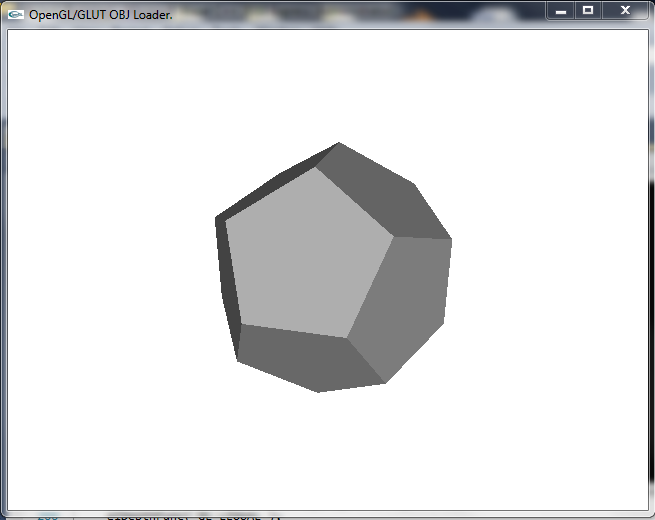
\includegraphics[max width=\textwidth]{pictures/screenshot-object-loader.png}
 \caption{Dvanásťsten načítaný zo súboru OBJ a vykreslený na obrazovku}
 \label{dodecahedron-render}
 \end{figure}

\section{Registrácia scény}

Na registráciu scény sme sa rozhodli použiť slobodnú knižnicu ARToolkit. Vznikla už v roku 1999 \cite{ARToolKit-b}, ale stále sa používa pre svoju jednoduchú rozšíriteľnosť. ARToolkit deteguje markery spôsobom popísaným v predchádzajúcej kapitole a nájde nám transformáciu, ktorou zarovnáme virtuálnu scénu v počítači do reálnej scény z~kamery.

Do tejto virtuálnej scény môžeme pomocou OpenGL vykresľovať to, čo potrebujeme. V prípade, že vieme aké bude osvetlenie fyzickej scény, môžeme podľa toho nastaviť osvetlenie vo virtuálnej scéne, aby neskutočné objekty pôsobili skutočnejšie.

Marker, ktorý používame na registráciu je priložený v prílohe A tejto práce. Na obrázku \ref{sova-marker} je ukážka modelu vykresleného na marker.

\begin{figure}[h]
 \centering
 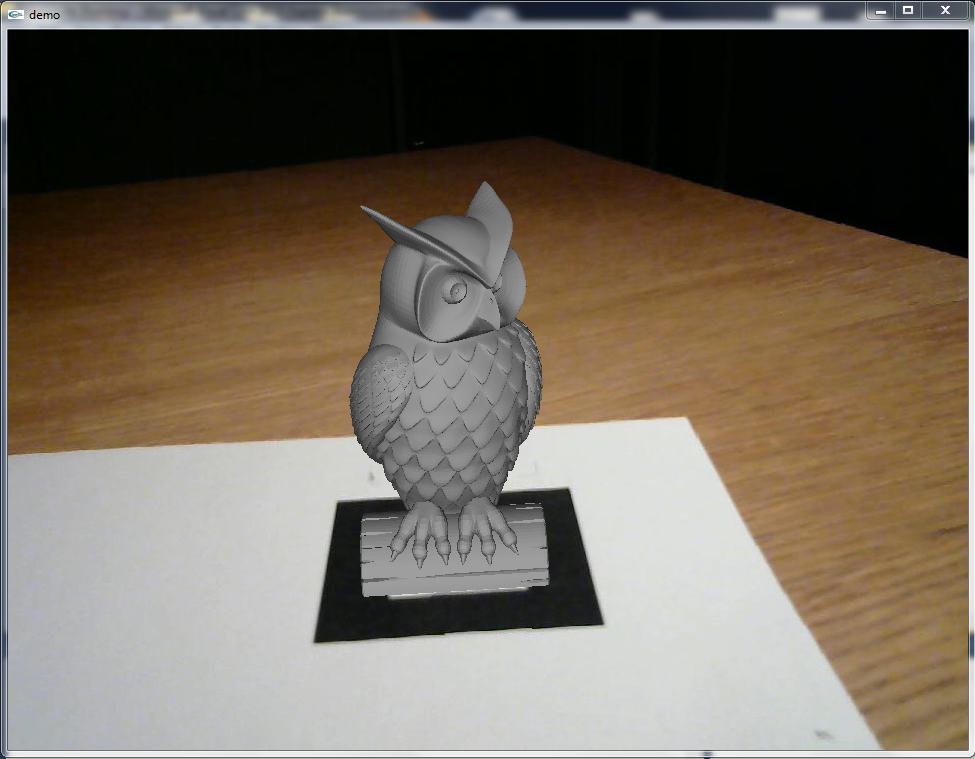
\includegraphics[max width=\textwidth]{pictures/screenshot-object.png}
 \caption{Model sovy vykreslený a umiestnený na marker v našej demo aplikácii}
 \label{sova-marker}
 \end{figure}

\section{Kalibrácia kamery}

Pokiaľ vytvárame aplikáciu s rozšírenou realitou dosiahnutou pomocou počítačového videnia a potrebujeme, aby zobrazovala virtuálne objekty čo najpresnejšie, je potrebné nakalibrovať kameru.

Kamery sa líšia kus od kusu a preto je potrebné vykonať meranie, ktorým získame parametre konkrétneho zariadenia. Tieto parametre potom zohľadníme pri rozpoznávaní obrazu.

V prípade bežnej dierkovej kamery (po anglicky \emph{pinhole camera}) sa tieto parametre usporiadavajú do matice parametrov kamery (\emph{camera matrix}), ktorá je vynásobením matice vnútorných (\emph{intrinsic}) parametrov s vonkajšími (\emph{extrinsic}) parametrami, ktoré udávajú transformáciu 3D súradníc svetu na 3D súradnice kamery. Určenie matice vnútorných parametrov kamery sa nazýva kalibrácia kamery.

\[
 A=
  \begin{pmatrix}
    \alpha_{x} & \gamma     & u_{0}\\
    0          & \alpha_{y} & v_{0}\\
    0          & 0          & 1
  \end{pmatrix}
\]

Matica vnútorných parametrov obsahuje parametre, ktoré sa dajú vypočítať nasledovne.

\begin{align}
\alpha_{x} = f \cdot m_{x} \\
\alpha_{y} = f \cdot m_{y}
\end{align}

Kde $m_{x}$ a $m_{y}$ sú škálovacie faktory pixelov a $f$ je ohnisková vzdialenosť. $\gamma$ je skresľovací koeficient medzi osami $x$ a $y$ a obvykle ho môžeme nastaviť na 0. $u_{0}$ a $v_{0}$ označujú posunutie optického stredu\footnote{Optický stred je bod, ktorý je prienikom optickej osi s priemetňou.} (po anglicky \emph{principal point}) v oboch osiach \cite{Hartley03}.

Tieto parametre je možné (pokiaľ sú známe vonkajšie parametre kamery) vypočítať z minimálne jednej fotky kalibračného vzoru\footnote{Obvykle sa pre zvýšenie presnosti použijú výsledky z viacerých fotiek vytvorených z rôznych uhlov. My sme ich pri kalibrácií vyhotovili dvadsať.}. Vhodné je fotiť napríklad šachovnicu alebo pole kruhov. Od začiatku merania nesmie kamera opticky preostrovať, ani meniť ohniskovú vzdialenosť (približovať), pretože by sa parametre zmenili.

Po transformácii maticou parametrov kamery vieme zvrátiť deformáciu obrazu.

\[
z_{c}\begin{bmatrix}
u\\
v\\
1\end{bmatrix}=A \begin{bmatrix}
R & T\end{bmatrix}\begin{bmatrix}
x_{w}\\
y_{w}\\
z_{w}\\
1\end{bmatrix}
\]

Pre kalibráciu kamery sme použili jednoduchý program využívajúci knižnicu pre~počítačové videnie OpenCV (obrázok \ref{kalib}). Táto knižnica implementuje šikovné metódy na detekciu kalibračnej siete aj výpočet parametrov z nameraných údajov. Taktiež umožňuje výpočet šošovkového skreslenia spôsobeného použitím bežnej kamery so šošovkou.

\begin{figure}[h]
 \centering
 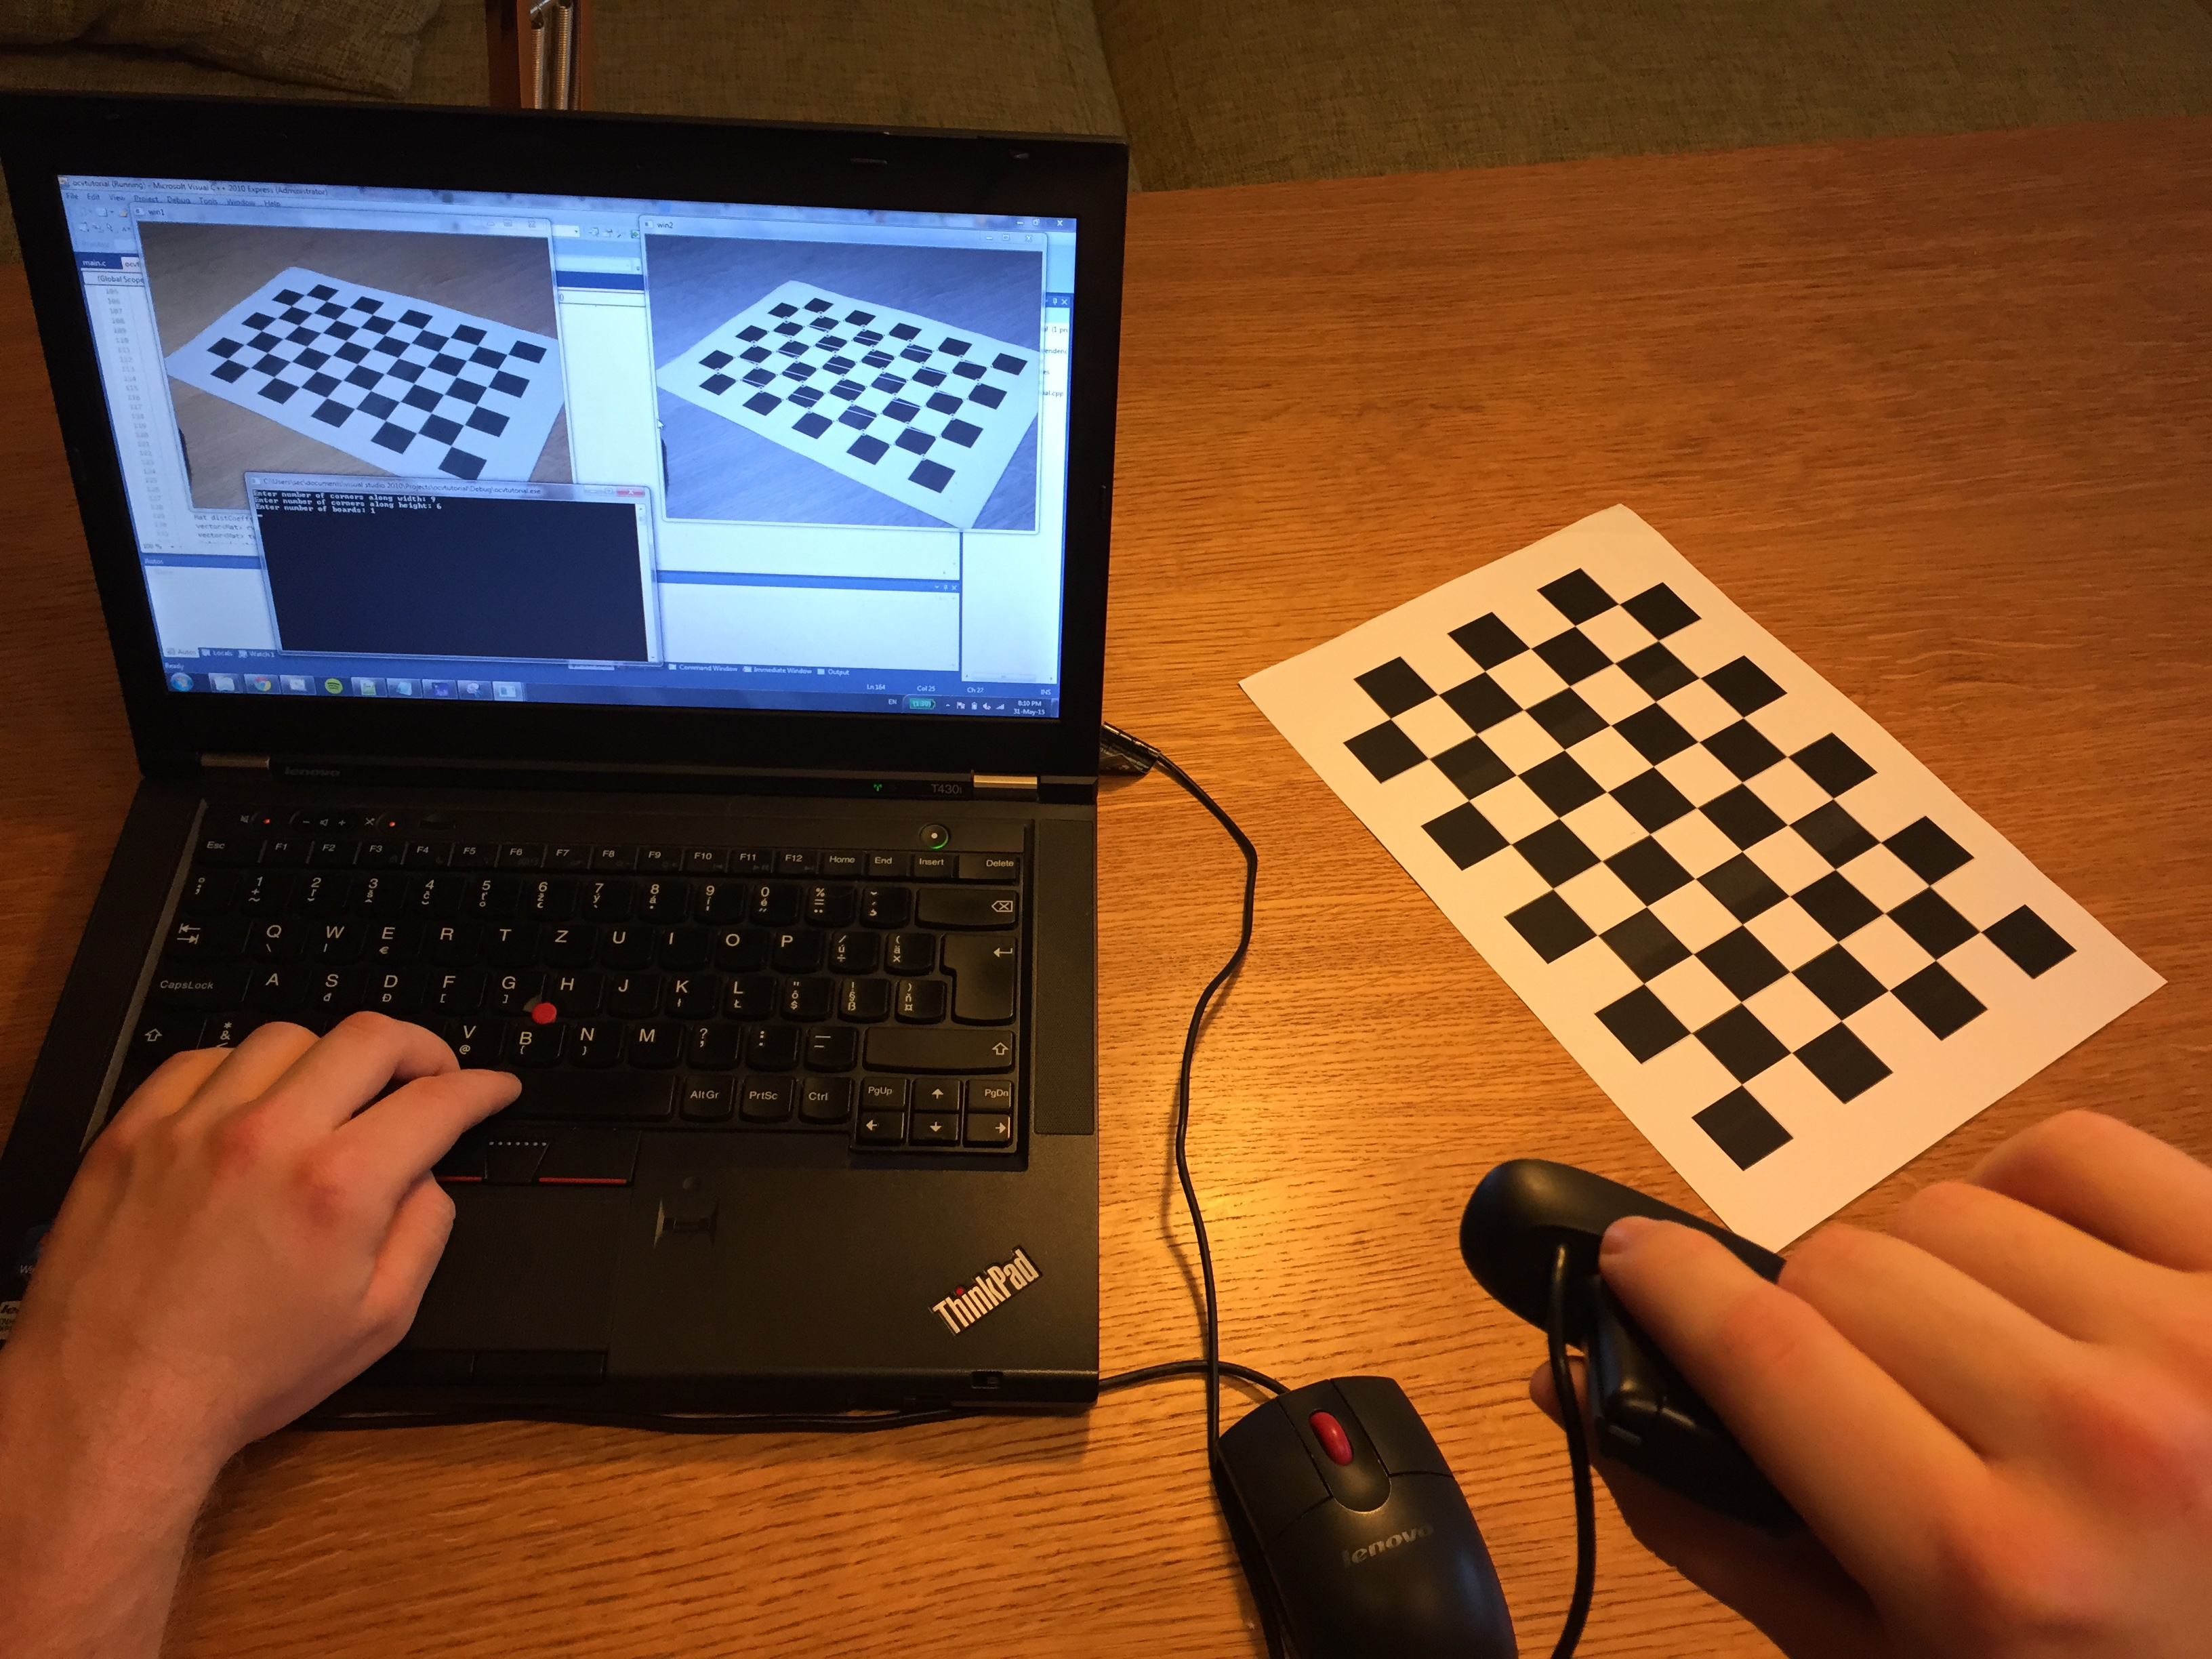
\includegraphics[max width=\textwidth]{pictures/kalibracia-foto.jpg}
 \caption{Kalibrácia kamery}
 \label{kalib}
 \end{figure}

\section{Príprava oklúderu}

Predtým ako môžeme implementovať oklúziu, potrebujeme mať vybraný oklúder a jeho digitálnu 3D reprezentáciu. Zvolili sme si na to viacero postupov.

\subsection{Modelovanie}

Najzákladnejší spôsob ako získať 3D model skutočného objektu, je ho jednoducho odmerať a vymodelovať v modelovacom programe. Pri prvom prototype ukázanom v článku \ref{section-prototyp} sme aplikovali zjednodušený postup a zvolili si za oklúder kocku, pretože má len osem vrcholov na jednoducho vymenovateľných súradniciach. Rozhodli sme sa vynechať načítavanie modelu a kocku popísať priamo v programe (znázornené na ukážke~\ref{kocka}). Vďaka tomu, že každé dve kocky sú si podobné stačí po popísaní kocky nájsť len správny škálovací koeficient.

\lstset{ %
  backgroundcolor=\color{myyellow},
  breakatwhitespace=false,         % sets if automatic breaks should only happen at whitespace
  breaklines=true,                 % sets automatic line breaking
  commentstyle=\color{dkgreen},    % comment style
  keepspaces=true,                 % keeps spaces in text, useful for keeping indentation of code (possibly needs columns=flexible)
  keywordstyle=\color{blue},       % keyword style
  language=C,                 % the language of the code
  otherkeywords={GL_GREATER, GL_KEEP, GL_STENCIL_TEST, GL_REPLACE, GL_ALWAYS, GLfloat},            % if you want to add more keywords to the set
  numbers=left,                    % where to put the line-numbers; possible values are (none, left, right)
  numbersep=5pt,                   % how far the line-numbers are from the code
  numberstyle=\tiny\color{gray}, % the style that is used for the line-numbers
  stepnumber=2,                    % the step between two line-numbers. If it's 1, each line will be numbered
  stringstyle=\color{mauve},     % string literal style
  tabsize=2,                       % sets default tabsize to 2 spaces
  caption={Reprezentácia kocky},                   % show the filename of files included with \lstinputlisting; also try caption instead of title
}

\begin{lstlisting}[label={kocka}]
	const GLfloat cube_vertices [8][3] = {
	{1.0, 1.0, 1.0}, {1.0, -1.0, 1.0}, {-1.0, -1.0, 1.0}, {-1.0, 1.0, 1.0},
	{1.0, 1.0, -1.0}, {1.0, -1.0, -1.0}, {-1.0, -1.0, -1.0}, {-1.0, 1.0, -1.0} };
	const short cube_faces [6][4] = {
	{3, 2, 1, 0}, {2, 3, 7, 6}, {0, 1, 5, 4}, {3, 0, 4, 7}, {1, 2, 6, 5}, {4, 5, 6, 7} };
\end{lstlisting}

\subsection{3D skener SMISS}

SMISS, teda \emph{Scalable Multifunctional Indoor Scanning System} je zariadenie vyvinuté na \emph{Fakulte matematiky, fyziky a informatiky Univerzity Komenského}, ktoré dokáže skenovať trojrozmerné objekty \cite{Kovacovsky13}. Objekt, ktorý je potrebné nasnímať sa položí na otočný stôl. Na tento stôl je pod uhlom namierená kamera a projektor. Projektor premieta na snímaný objekt štruktúrované svetlo. Toto svetlo projektuje pruhy, ktorými „rozreže“ skenovaný objekt na jednotlivé roviny, pričom každá rovina je osvetlená a zakódovaná iným vzorom svetla. Každé nasvietenie je odfotené kamerou. Na začiatku skenovania je objekt rozdelený iba na zopár rovín, tie sa ale postupne delia na tenšie rezy, čím vzniká vyššia detailnosť. Keď sú nasnímané všetky požadované nasvietenia, motor stôl pootočí a projektor začne objekt znovu nasvecovať z nového uhlu \cite{Kovacovsky12-a, Kovacovsky12-b}.

Počítač z obrazu dekóduje jednotlivé roviny a po zosnímaní zo všetkých strán vytvorí mračno bodov (po anglicky \emph{point cloud}) reprezentujúce objekt. Na výsledné mračno bodov môžeme aplikovať trianguláciu a tým získame polygonálny model, ktorý môžeme použiť ako oklúder. Priemerná prestnosť SMISSu je \SI{500}{\micro\metre} \cite{Kovacovsky12-b}.

Na skeneri sme skenovali lepiacu pásku, ktorá je na obrázku \ref{paska} a výsledok jej skenovania je na obrázku \ref{paska-cloud}.

\begin{figure}[h]
 \centering
 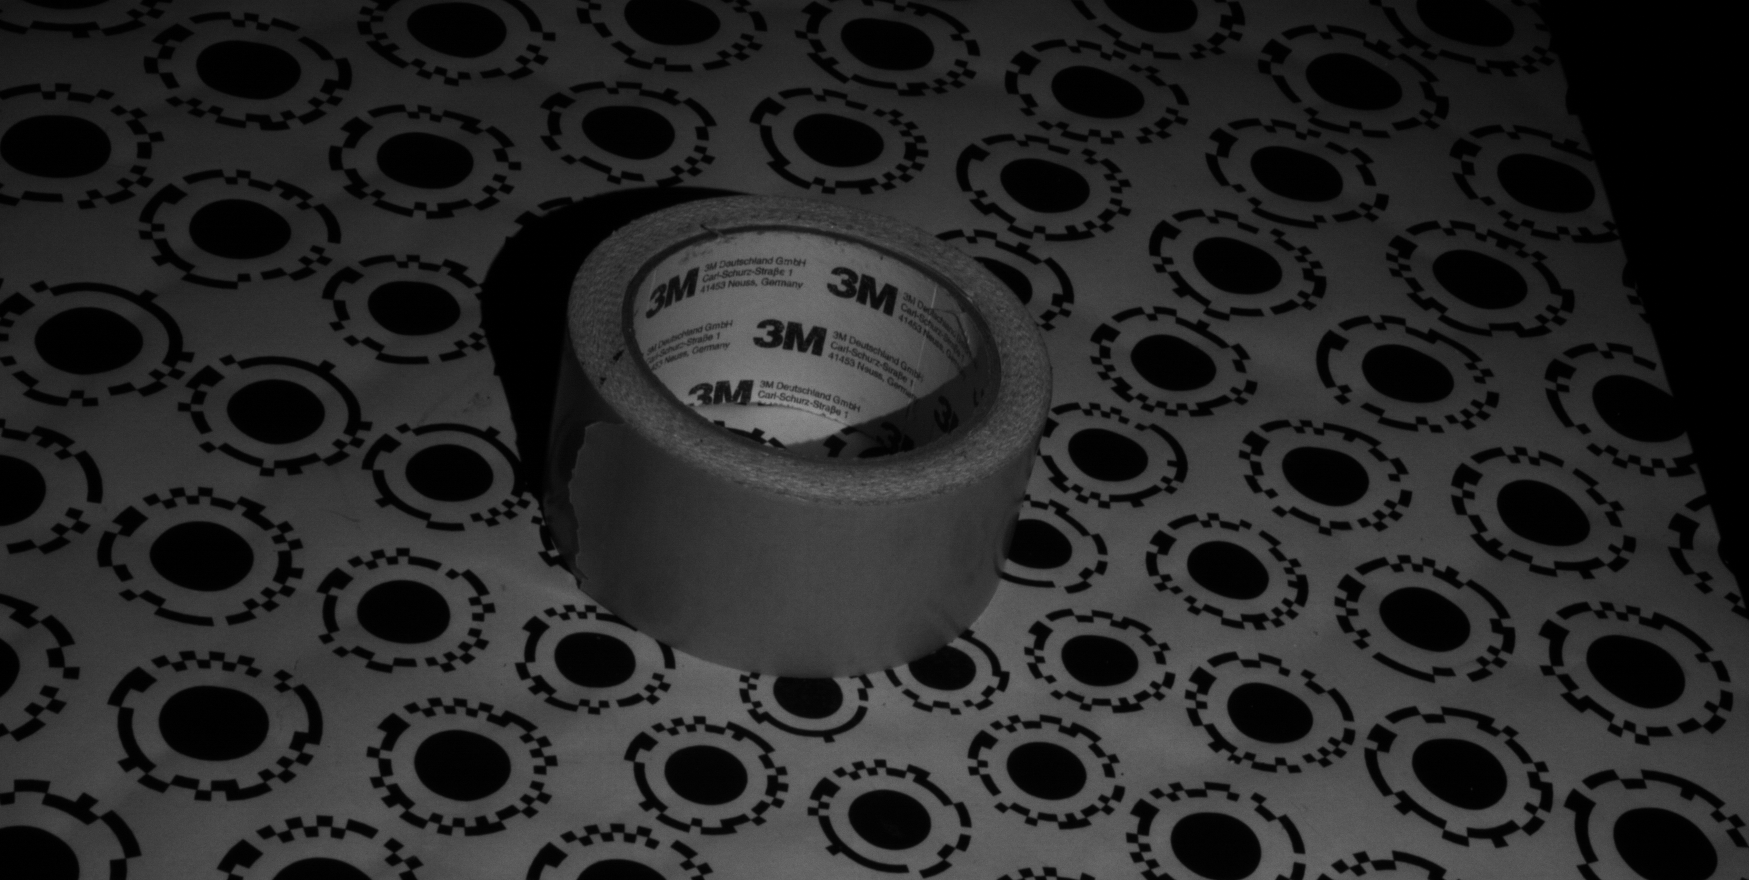
\includegraphics[max width=\textwidth]{pictures/smiss.png}
 \caption{Lepiaca páska z pohľadu skeneru SMISS}
 \label{paska}
 \end{figure}

\begin{figure}[h]
 \centering
 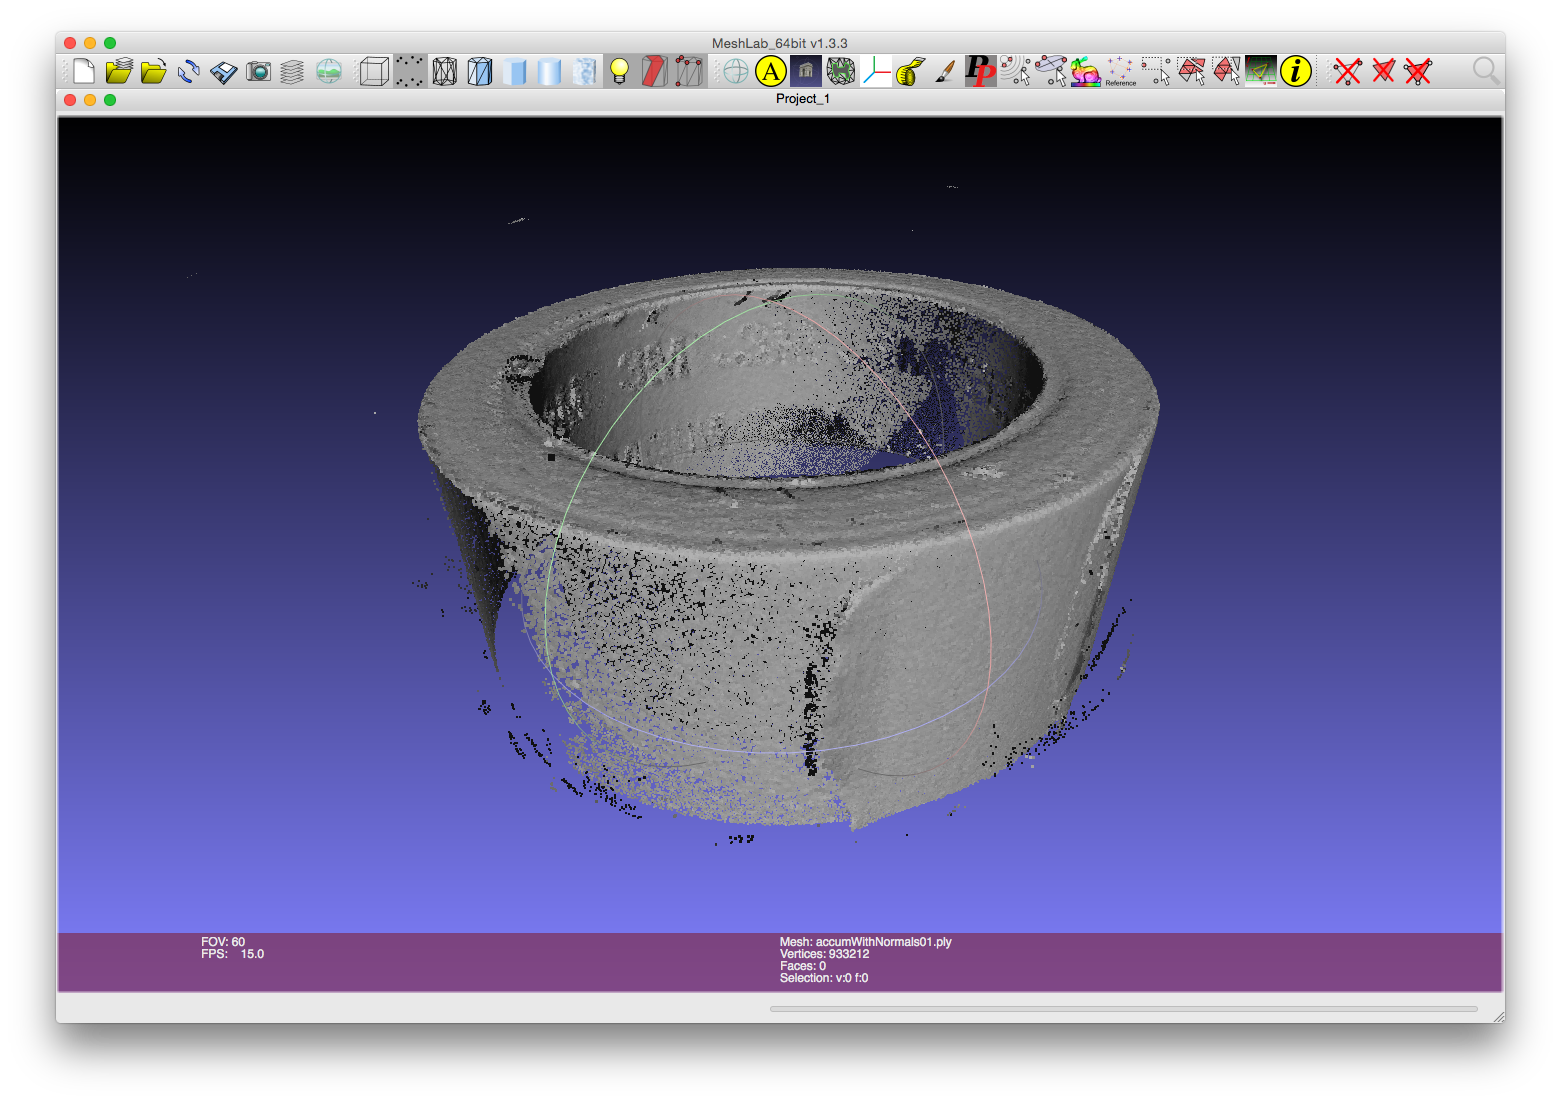
\includegraphics[max width=\textwidth]{pictures/smiss-pointcloud.png}
 \caption{Mračno bodov, ktoré je výstupom skenovania SMISSom}
 \label{paska-cloud}
 \end{figure}

\subsection{3D tlač}

Druhou možnosťou, ako získať oklúder a jeho virtuálny 3D model je namodelovať ho v~počítači a potom ho vytlačiť na 3D tlačiarni. Na vytvorenie takéhoto modelu je vhodný napríklad Blender, z ktorého ho potom môžeme vyexportovať do OBJ pre~aplikáciu aj STL pre tlač.

STL model nahráme do \emph{slicera}, to je program, ktorý zoberie model a ‚rozreže‘ ho na~veľký počet 2D vrstiev. Príkladom je slicer MakerBot Desktop, dodávaný k~tlačiarňam značky MakerBot. Výška vrstvy závisí od nastaveného rozlíšenia. Tieto dáta sa potom vložia do tlačiarne a tá začne roztápať plastovú náplň (\emph{fillament}) a~nanášať ju vrstvu po vrstve na seba.

Inteligentný slicer dokáže do dutého modelu dorobiť sieť vnútorných stien, aby sa nerozpadol. V prípade, že tlačený predmet obsahuje časti, ktoré prevísajú von a teda by ich nebolo ako tlačiť do vzduchu, môže slicer dopočítať podpery, ktoré sa vytlačia spolu s modelom a po vytlačení sa odrežú. V prípade použitia tlačiarne s dvomi tlačiacimi hlavami je dokonca možné použiť dva fillamenty, z toho jeden vodou rozpustný, ktorým sa tlačia podpery. Po tlači sa model len ponorí do vody.

Dnešné 3D tlačiarne zvládajú rozlíšenie okolo \SI{100}{\micro\metre}, čo je okolo 255 dpi, teda 255 vrstiev na jeden palec výšky. Nevýhodou je, že s kvalitou rýchlo narastá aj čas, ktorý tlačenie potrvá.

Na tlačiarni sme tlačili model sovy z obrázku \ref{sova-blend} a jej výtlačok je na obrázku \ref{sova-print}.

\begin{figure}[h]
 \centering
 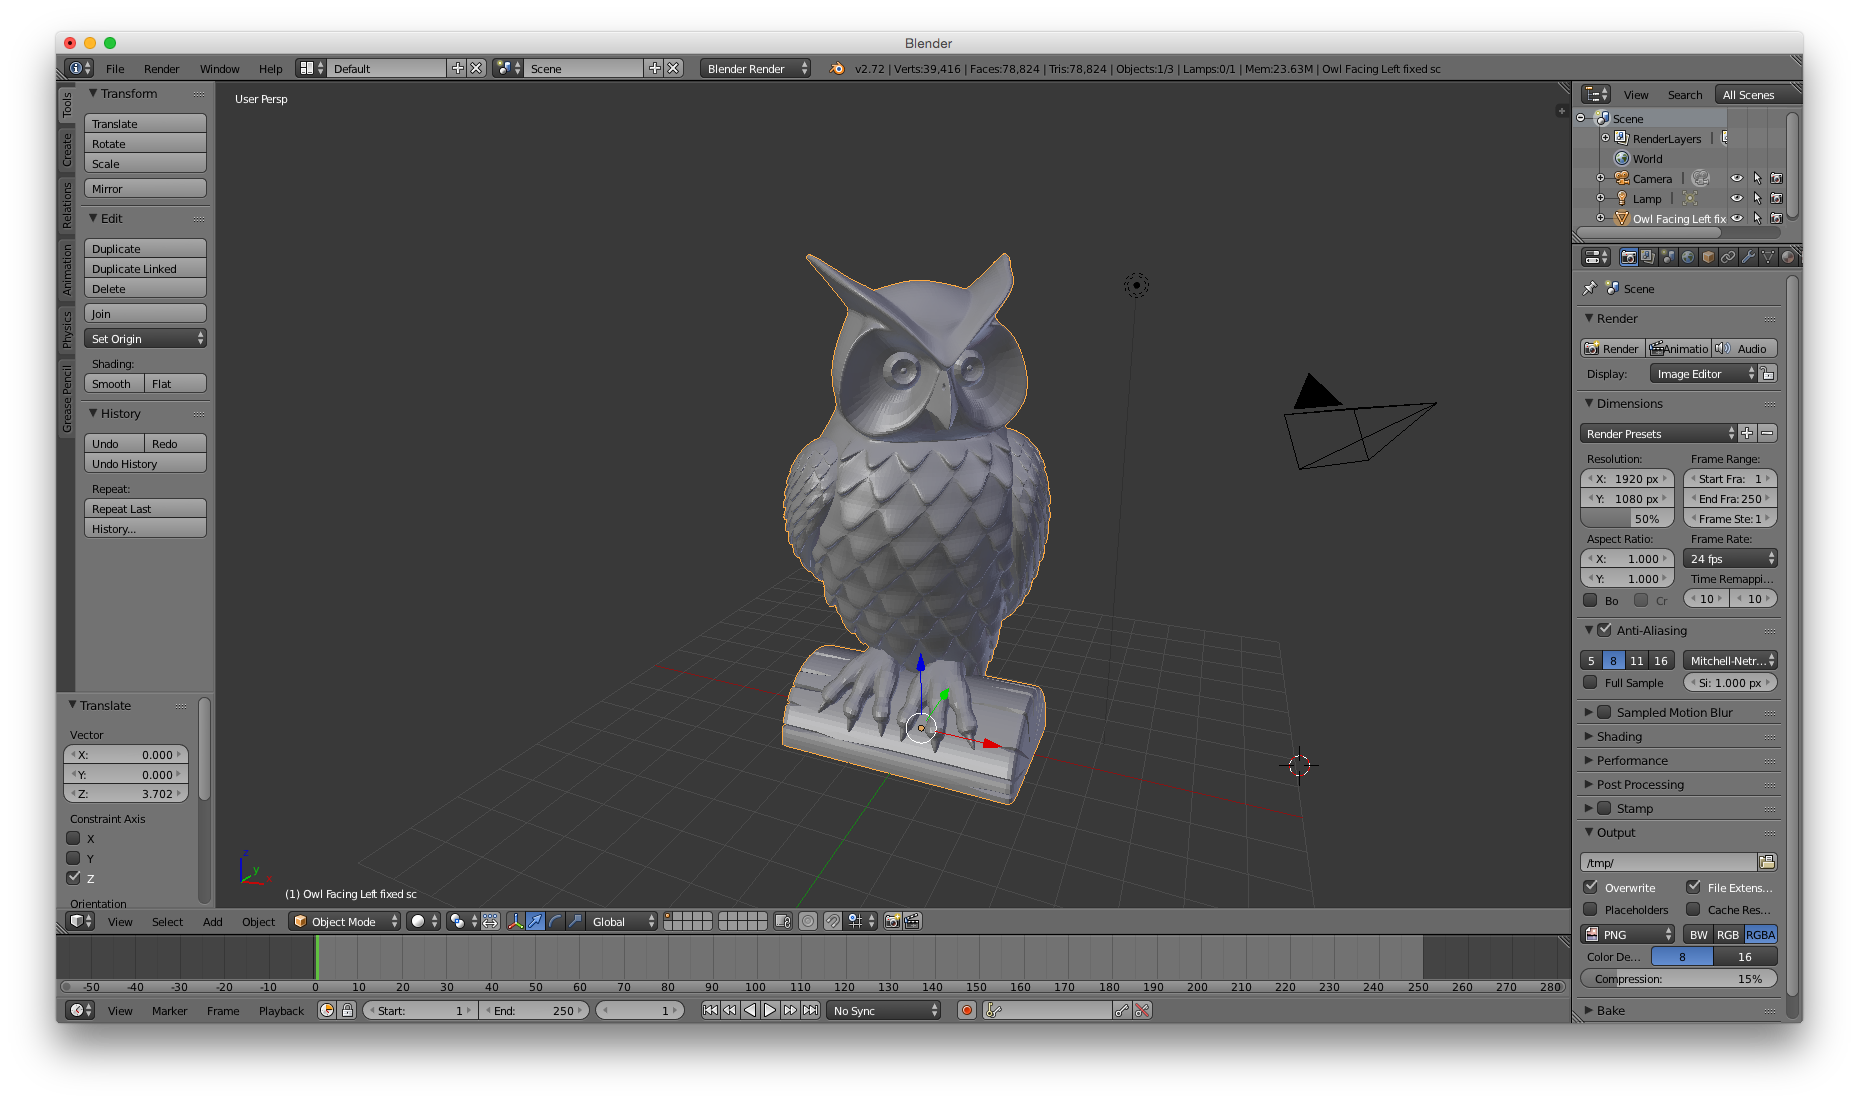
\includegraphics[max width=\textwidth]{pictures/owl-blender.png}
 \caption{Digitálny model sovy, otvorený v modelovacom programe Blender. Autorom modelu je modelár Tom Cushwa \cite{Cushwa}}
 \label{sova-blend}
 \end{figure}

\begin{figure}[h]
 \centering
 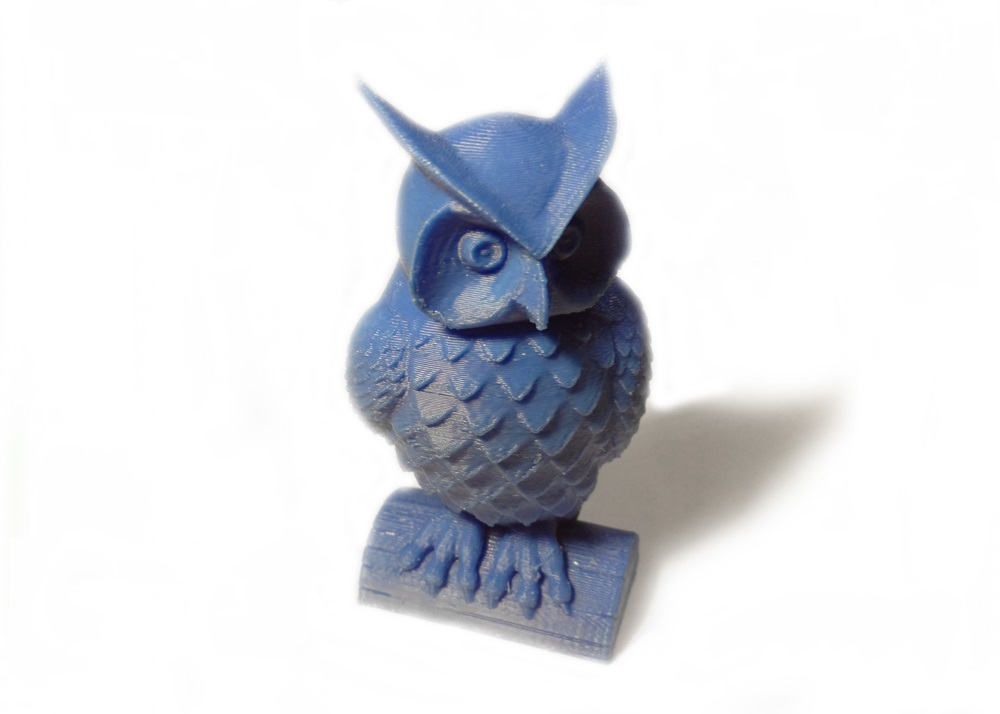
\includegraphics[max width=\textwidth]{pictures/owl-model.jpg}
 \caption{Fyzický model sovy, ktorý sme vytlačili na 3D tlačiarni}
 \label{sova-print}
 \end{figure}

\section{Oklúzia v rozšírenej realite}

Ak chceme v rozšírenej realite zobrazovať virtuálne objekty tak, aby ich úplne, alebo čiastočne prekrývali fyzické objekty na scéne, je potrebné, aby pre každý tento fyzický objekt aplikácia okrem virtuálneho 3D modelu poznala aj jeho veľkosť a polohu na~scéne voči markeru, prípadne ho vedela inak rozoznať.

Program následne objekty, prípadne ich časti, ktoré sú prekryté oklúderom ne\-vy\-kres\-lí a rovnako ne\-vy\-kres\-lí ani samotný oklúder. Na mieste, kde majú byť objekty prekryté sa teda zobrazí stopa z videa, ktorá je na pozadí. Táto stopa na danom mieste obsahuje pôvodný fyzický objekt zosnímaný kamerou a tým sa vytvorí ilúzia, že virtuálne objekty sú prekryté tými reálnymi. Pri oklúzií je obzvlášť dôležité mať správne nakalibrovanú kameru, aby sa virtuálne objekty premietali čo najpresnejšie na~svoje miesta.

Najprv si vykreslíme pomocou OpenGL oklúder do \emph{stencil bufferu}. Tento buffer je binárnym obrázkom veľkosti vykresľovaného okna a slúži ako úložné miesto na dočasné informácie o danom obraze. Na každý bod v stencil bufferi zapíšeme true, pokiaľ by sa na dané súradnice v normálnom pohľade vykreslila časť oklúdera. Neskôr pri~vykresľovaní virtuálnych objektov, ktoré sa majú nachádzať za oklúderom, robíme pre~každý pixel jednoduchú kontrolu. Nachádza sa na týchto súradniciach v stencil bufferi hodnota true? Ak sa nachádza, tak pixel nevykreslíme, pretože nemá byť vidieť a~pokračujeme ďalej. Táto logika je znázornená na ukážke \ref{okluzia-kod}.

\lstset{ %
  backgroundcolor=\color{myyellow},
  breakatwhitespace=false,         % sets if automatic breaks should only happen at whitespace
  breaklines=true,                 % sets automatic line breaking
  commentstyle=\color{dkgreen},    % comment style
  keepspaces=true,                 % keeps spaces in text, useful for keeping indentation of code (possibly needs columns=flexible)
  keywordstyle=\color{blue},       % keyword style
  language=C,                 % the language of the code
  otherkeywords={GL_GREATER, GL_KEEP, GL_STENCIL_TEST, GL_REPLACE, GL_ALWAYS, GLfloat},            % if you want to add more keywords to the set
  numbers=left,                    % where to put the line-numbers; possible values are (none, left, right)
  numbersep=5pt,                   % how far the line-numbers are from the code
  numberstyle=\tiny\color{gray}, % the style that is used for the line-numbers
  stepnumber=2,                    % the step between two line-numbers. If it's 1, each line will be numbered
  stringstyle=\color{mauve},     % string literal style
  tabsize=2,                       % sets default tabsize to 2 spaces
  caption={Implementácia oklúzie},                   % show the filename of files included with \lstinputlisting; also try caption instead of title
}

\begin{lstlisting}[label={okluzia-kod}]
//render occluder to stencil buffer
glEnable(GL_STENCIL_TEST);
glStencilOp(GL_REPLACE, GL_REPLACE, GL_REPLACE);
glStencilFunc(GL_ALWAYS, 1, 0xffffffff);
DrawOccluder();

//render occluded object
glStencilFunc(GL_GREATER, 1, 0xffffffff);
glStencilOp(GL_KEEP, GL_KEEP, GL_KEEP);
DrawObject();
glDisable(GL_STENCIL_TEST);
\end{lstlisting}

\section{Výsledky}

Aplikácia má funkcionalitu, ktorú sme si špecifikovali. Na obrázku \ref{scene} je znázornený príklad scény na ktorej predvádzame aplikáciu. Na obrázku \ref{no-occlusion} je snímka obrazovky z aplikácie v situácií, kedy registrujeme scénu, ale oklúder neprekrýva vykreslovaný objekt\footnote{Autorom voľne šíriteľného modelu stromu v pozadí je theswiss z portálu Thingiverse \cite{theswiss14}.} a k oklúzií preto nedochádza.

\begin{figure}[h]
 \centering
 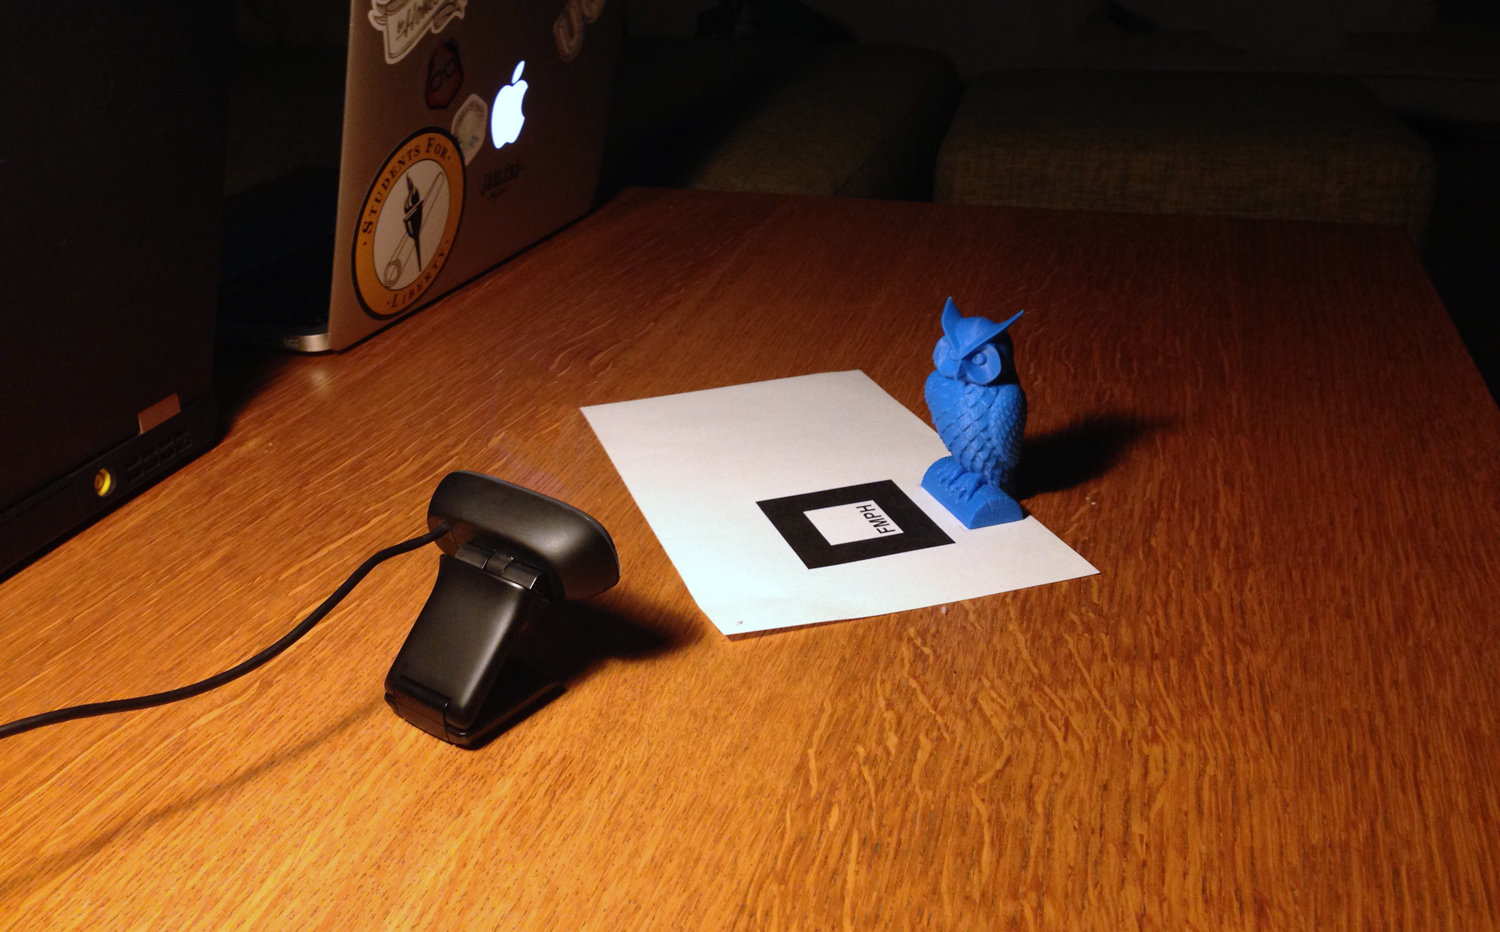
\includegraphics[max width=\textwidth]{pictures/scene.jpg}
 \caption{Scéna na ktorej demonštrujeme oklúziu. Modrý model sovy je oklúderom.}
 \label{scene}
 \end{figure}

\begin{figure}[h]
 \centering
 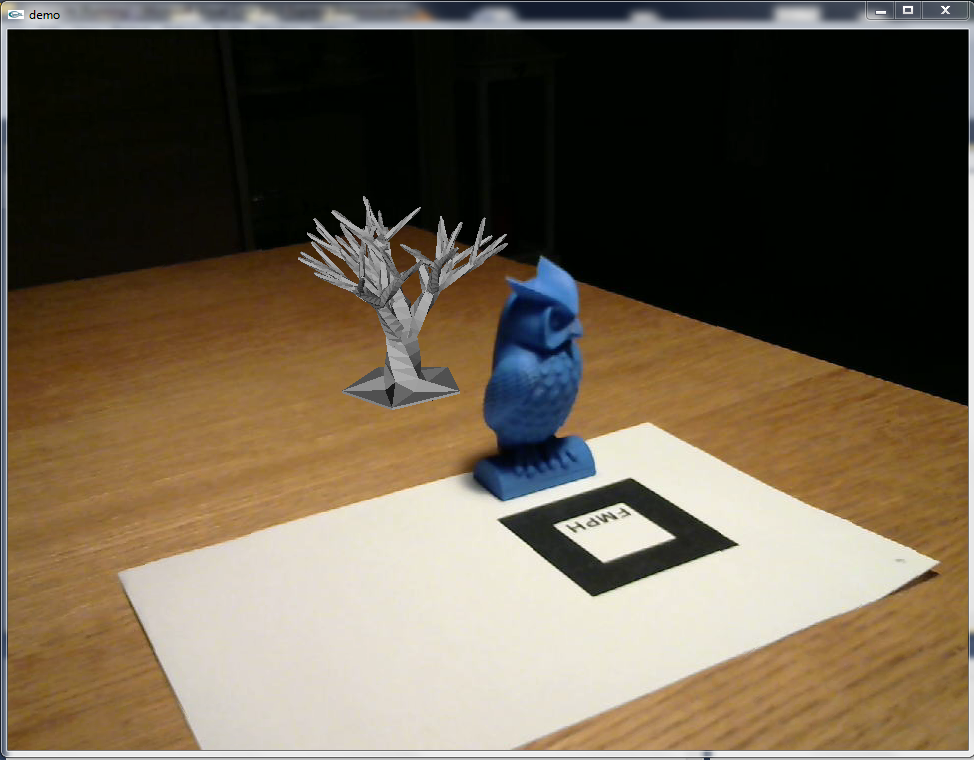
\includegraphics[max width=\textwidth]{pictures/screenshot-separate.png}
 \caption{Skutočný a virtuálny objekt sa neprekrývajú, takže k oklúzii nedochádza}
 \label{no-occlusion}
 \end{figure}

Aby sme sa uistili, že máme fyzický oklúder položený na správnu relatívnu pozíciu voči markeru, môžeme si v aplikácii zapnúť vykresľovanie oklúderu a pozrieť sa, nakoľko presne sa prekrývajú (znázornené na obrázku \ref{show-occluder}).

Ak je oklúder správne zarovnaný a vypneme jeho vykresľovanie na obrazovku, dosiahneme oklúziu, ako je vidno na obrázku \ref{true-occlusion}.

\begin{figure}[h]
 \centering
 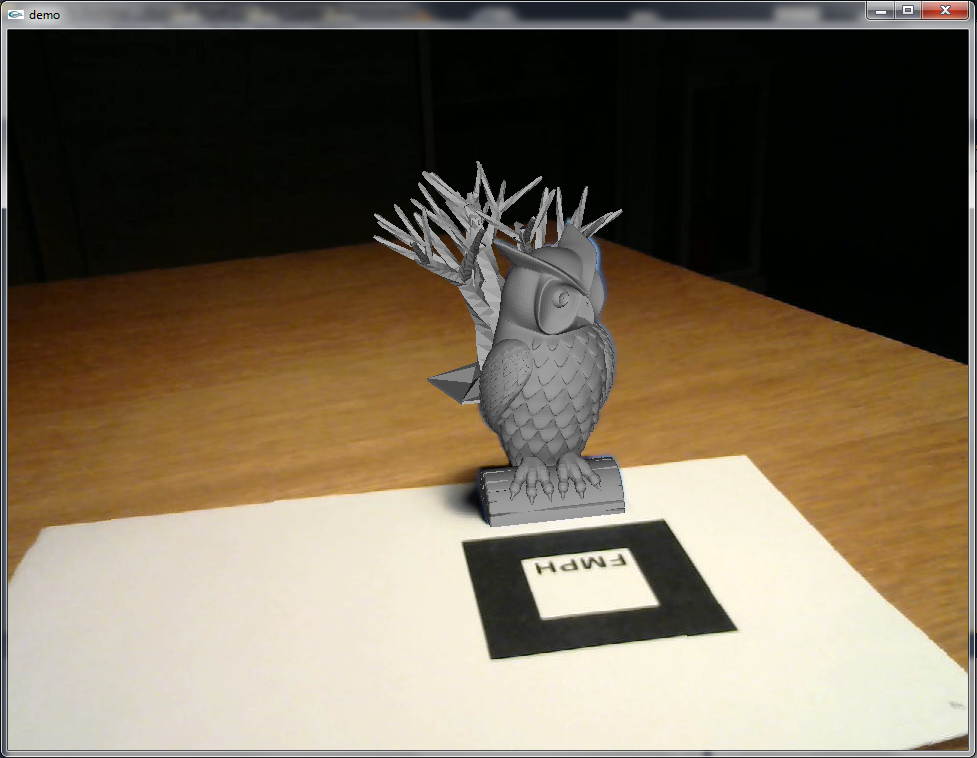
\includegraphics[max width=\textwidth]{pictures/screenshot-occluder.png}
 \caption{Natočili sme scénu tak, aby sa objekty prekrývali a nechali sme vykreslovať aj virtuálny model oklúderu, ktorý sa pomocou markeru registruje cez skutočnú sovu.}
 \label{show-occluder}
 \end{figure}

\begin{figure}[h]
 \centering
 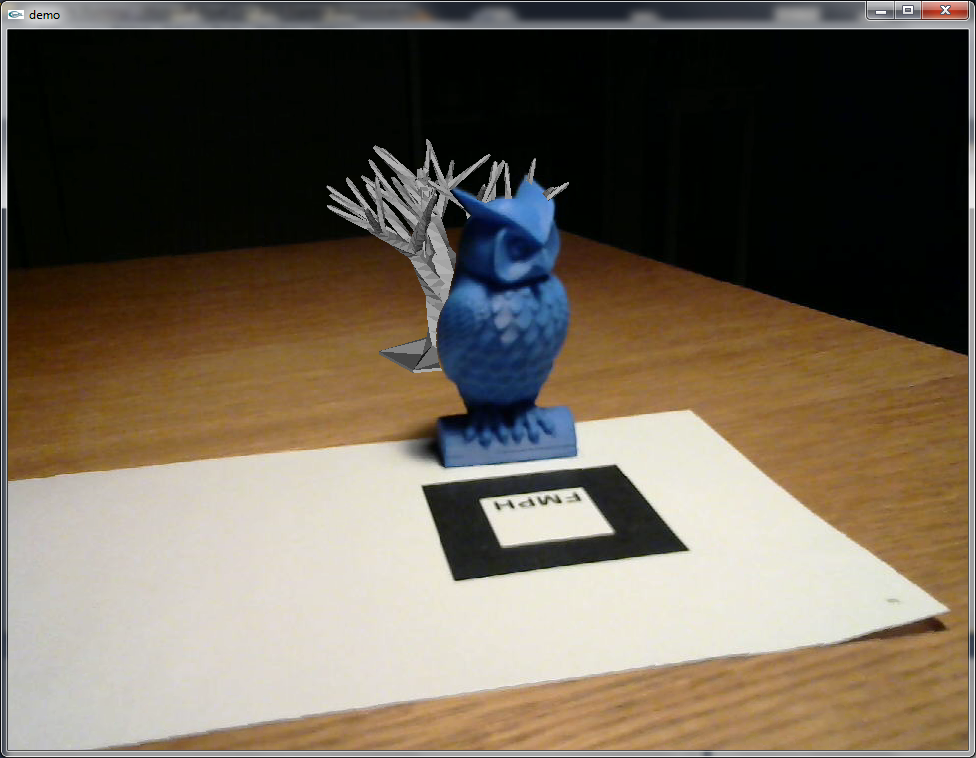
\includegraphics[max width=\textwidth]{pictures/screenshot-occlusion.png}
 \caption{V predchádzajúcej scéne sme nechali oklúder vykresľovať iba do stencil bufferu a výsledkom je oklúzia s fyzickým objektom.}
 \label{true-occlusion}
 \end{figure}
 
 \subsection{Výkon aplikácie}
 
 Bez ohľadu na zložitosť (počet vrcholov) skúšaných modelov nám aplikácia bežala na našom hardvéri plynulo pri framerate 29 až 30 snímkov za sekundu (\emph{framerate} vyjadruje rýchlosť obnovovania obrazovky). Informácie o použitých modeloch sú uvedené v tabuľke 4.1. Na obrázku \ref{benchmark} sú vykreslené všetky modely naraz, tiež pri framerate 30 snímkov za sekundu.
  
 Hodnota 30 snímkov za sekundu je limitovaná našou kamerou, ktorá nezvláda robiť snímky rýchlejšie a aplikácia teda musí po spracovaní snímku čakať na nasledovný snímok.
 
 Aplikáciu sme spúšťali na počítači s procesorom Intel Core i3 taktovaným na 2.4 GHz, 8 GB pamäte a integrovanou grafickou kartou Intel HD 3000. Snímky z kamery boli spracovávané v rozlíšení 960 na 720 pixelov.
 
 \begin{center}
   \begin{tabular}{| l | r | r |}
     \hline
     model &  počet vrcholov &  počet stien \\ \hline\hline
     sova (oklúder) & 39416 & 7824 \\ \hline
     loď Enterprise & 2680 & 5372 \\ \hline
     drak Alduin & 8160 & 16074 \\ \hline
     mesto Atlantis & 41437 & 83190 \\ \hline \hline
     spolu & 91693 & 112460 \\ \hline
   \end{tabular}
   \captionof{table}{Údaje o modeloch použitých pri testovaní výkonu aplikácie} 
 \end{center}
 
\begin{figure}[h]
 \centering
 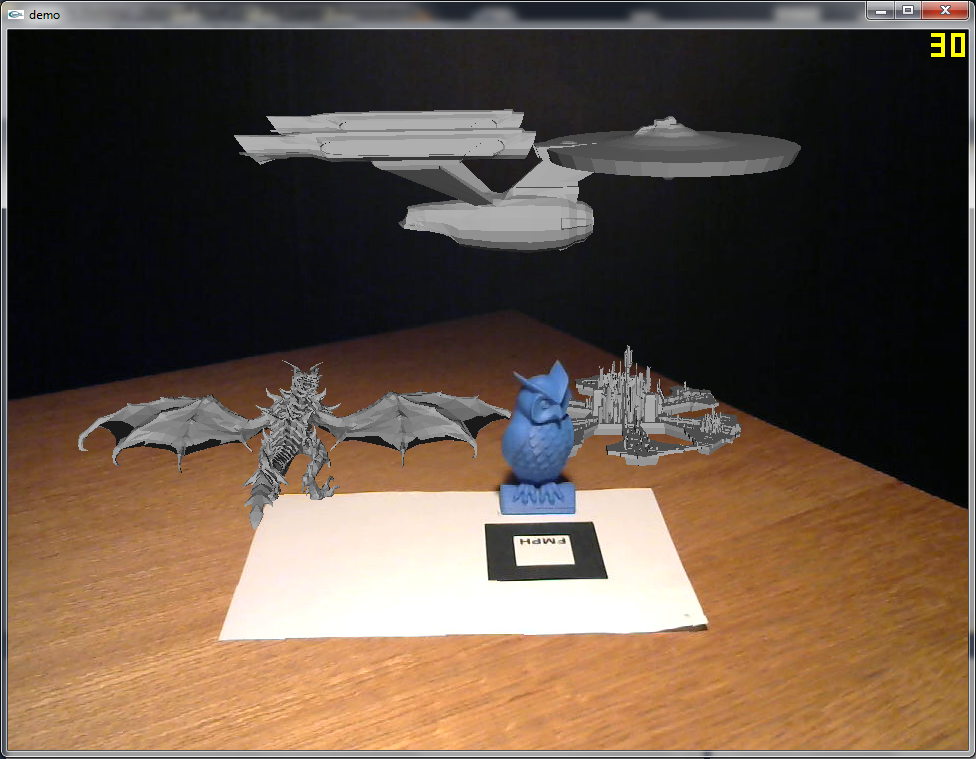
\includegraphics[max width=\textwidth]{pictures/benchmark.png}
 \caption{Vykresľovanie viacerých modelov naraz}
 \label{benchmark}
 \end{figure}
 
 \subsection{Možné problémy a nepresnosti}
 
 Detekcia markeru funguje spoľahlivo a aplikácia obvykle nemá problémy s identifikáciou scény pokiaľ je celý marker viditeľný. Zaznamenali sme iba jeden prípad kedy detekcia zlyhá a to keď je časť markeru v tieni. Táto situácia môže ľahko nastať, pokiaľ je scéna nasvietená ostrým svetlom (napríklad stolnou lampou) spoza oklúderu a oklúder zatieňuje časť markeru.
 
 Problémy s nepresnosťou oklúzie môžu nastať niekoľkými spôsobmi, prípadne ich kombináciou. Fyzický model oklúderu je potrebné relatívne umiestniť voči markeru veľmi presne, čo môže byť obtiažne. Nepresnosť taktiež môže spôsobiť nesprávne naškálovaný virtuálny model oklúderu. Nenakalibrovaná, alebo nedostatočne presne nakalibrovaná kamera spôsobuje ďaľšiu nepresnosť. Tieto nepresnosti sa prejavujú tak, že výrez vo vykresľovanom objekte je posunutý oproti fyzickému oklúderu a nie je s~ním presne zarovnaný.
\chapter{Budúcnosť rozšírenej reality}
\def\thepage{\textit{\arabic{page}}}

Cena zariadení, na ktorých sa dá vytvárať rozšírená realita sa neustále znižuje, zatiaľ čo ich výkon sa rapídne zvyšuje. Pred dvadsiatimi rokmi si bolo možné vyskúšať rozšírenú realitu iba na drahých zariadeniach vo výskumných laboratóriach. Vďaka tomu, že na sprostredkovanú rozšírenú realitu postačí počítač
s kamerou, sa dostupnosť a rozšírenie týchto zariadení zväčšuje. Ľudia si nekupujú zariadenia preto, aby s nimi používali rozšírenú realitu, ale kupujú si zariadenia,
ako sú chytré telefóny a tablety, ktoré dokážu spúšťať rozšírenú realitu, aj keď to nie je ich primárny účel. Počítače sa postupne dostávajú do stále väčšieho množstva chytrých zariadení. Z javu všadeprítomných počítačov (po anglicky \emph{ubiquitus computing}) by mohla rozšírená realita veľa vyťažiť~\cite{Zhou08}.

Rozšírená realita má už dnes množstvo praktických využití, väčšina z nich je ale veľmi špecifická, určená pre úzku skupinu ľudí, alebo veľmi konkrétnu úlohu. Na to, aby sa rozšírená realita v budúcnosti používala viac, je potrebné
vyvinúť všeobecnejšie a praktickejšie aplikácie.

\section{Nové zariadenia}

Veľké pokroky v miniaturizácii len posledné desaťročie umožnili praktické používanie nositeľných počítačov (po anglicky \emph{wearable computers}), teda počítačov, ktoré používateľ nosí na svojom tele tak, ako oblečenie. Koncept okuliarov s rozšírenou realitou existuje už desaťročia, ale ešte donedávna boli všetky helmy vyrobené na tento účel príliš ťarbavé. Počítače, displeje a kamery boli väčšie, nepresnejšie a potrebovali viac energie. Batérie boli ťažšie a zaberali viac priestoru. Helmy s rozšírenou realitou najprv pokrývali celú hlavu, boli ťažké a obmedzovali používateľa pri pohybe. Zo začiatku k~nim bolo potrebné nosiť ruksak, v ktorom sa ukrýval počítač a batérie. Tieto helmy sa postupne zmenšovali, až sa zmenili na okuliare, ale žiadne z nich nedosiahli úroveň, ktorá by mohla dosiahnuť komerčného úspechu a rozšíriť používanie. Pri nositeľných počítačoch je používanie ovplyvnené aj módou. Tieto zariadenia musia vyzerať dobre a ich používatelia sa nesmú cítiť divnými.

\subsection{Google Glass}

Jednými z okuliarov, ktorým by sa mohlo podariť stať sa používanými na verejnosti sú Google Glass. Glass sú futuristické okuliare od Googlu, ktoré majú v ráme zabudovanú malú batériu, počítač, kameru a projektor, ktorý premieta obraz na sklenený hranol pred okom používateľa (sú znázornené na obrázku \ref{glass}). Na rozšírenú realitu nie sú zrovna ideálne, pretože tento hranol je iba v pravom hornom rohu pravého oka, zobrazovacia plocha teda pokrýva iba malú časť zorného pola \cite{Google14-b}. Napriek tomu sa na nich dá rozšírená realita aplikovať — napríklad firma Layar pre ne vytvorila svoju aplikáciu, ktorá používateľovi na domy, na ktoré sa pozerá umiestňuje v prípade, že sú na predaj ikonky a zobrazuje ich stránky v realitných kanceláriach \cite{LayarAR}. Táto aplikácia ale beží iba v rohu užívateľovho zorného pola a domy, ktoré sa v tejto zóne nenachádzajú ignoruje, pretože nemá možnosť na ne ikonky vykresliť. V januári 2015 Google ukončil experimentálnu fázu projektu a prisľúbil, že pracuje na novej verzií.

\begin{figure}[h]
 \centering
 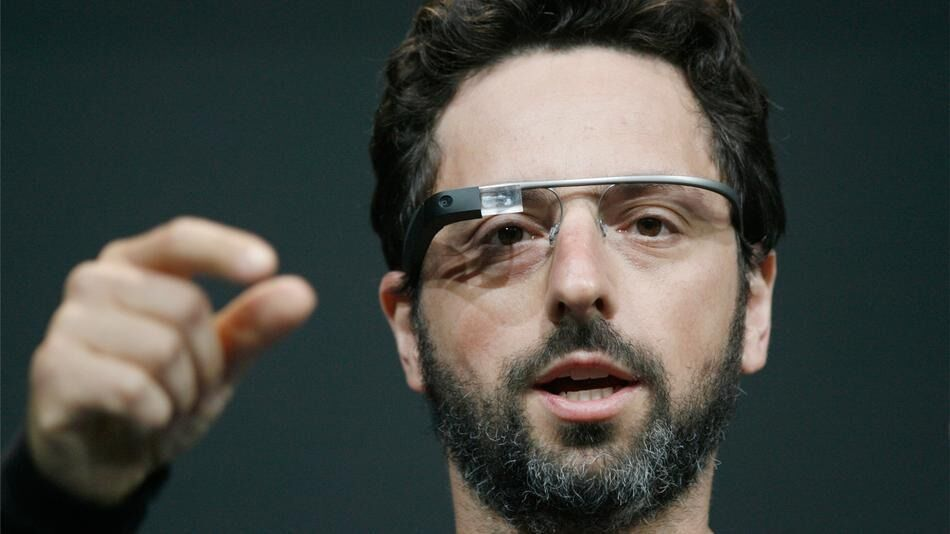
\includegraphics[max width=\textwidth]{pictures/bringlass.jpg}
 \caption{Spoluzakladateľ Google, Sergej Brin demonštruje Google Glass; autor: Kimihiro Hoshino}
 \label{glass}
 \end{figure}

Google Glass nie sú dôležité preto, že by to boli okuliare, ktoré sú dobre uspôsobené na rozšírenú realitu — to nie sú. Sú dôležité preto, že majú potenciál stať sa v budúcnosti komerčne rozšírenou platformou, ktorá môže naštartovať celé nové technologické odvetvie chytrých okuliarov. Práve tak ako chytré telefóny nie sú určené na rozšírenú realitu a napriek tomu sú na ňu používané viac ako zariadenia špeciálne vyvinuté len pre rozšírenú realitu, by sa mohli aj Google Glass, nevyvíjané primárne pre rozšírenú realitu stať budúcou klasickou platformou pre šírenie tejto technológie.

\def\thepage{\arabic{page}}
\subsection{Eyeborg}

Kanaďan Rob Spence prišiel pri nehode o pravé oko. Svojpomocne si skonštruoval protézu s bezdrôtovou kamerou, ktorú odvtedy vylepšuje. Cez toto robotické oko nevidí - zatiaľ sa z neho video odosiela do iného zariadenia, na ktorom sa dá prehrávať. Tento systém obsahuje rozšírenú realitu a dokáže rozoznávať vo videu objekty a manipulovať s~nimi \cite{Eyeborg}. Momentálne musí používateľ pozerať svojim zdravým okom na displej a svalmi v pravej očnej dutine ovláda kameru. Na výskume v oblasti umelého zraku sa pracuje a sú prípady, keď sa podarilo pacientom napojiť signál z kamery na optický nerv a navrátiť im veľmi obmedzené videnie \cite{Dobelle00}. Až sa podobné operácie stanú úplne bežnými, tieto bionické oči budú ideálnou platformou na rozšírenú realitu.

\section{Uchytenie v bežnom živote}

Ukazuje sa, že oblasť je už zrejme dostatočne vyspelá na to, aby bola použiteľná v~bežnej praxi. Nový hardvér umožňuje využívať rozšírenú realitu viac luďom ako kedykoľvek predtým. Jednou z otázok súčastnosti je aj to, či sa tento koncept naozaj presadí v bežnom živote.

V období okolo roku 2009 malo veľké množtvo ľudí svoje prvé chytré mobilné telefóny. V tom čase vzniklo množstvo aplikácií, ktoré využívali rozšírenú realitu rôznymi spôsobmi. Jednou z týchto aplikácií boli napríklad aj slovenské Zlaté Stránky, ktoré na obrazovku telefónu do obrazu z kamery dopisovali názvy firiem na miesta, kde sídlia~\cite{Orgonas10}. Tieto aplikácie sa staly okamžitým hitom, pretože väčšina používateľov si na nich mohla vyskúšať rozšírenú realitu po prvýkrát. Ich popularita však postupne klesla, ako je vidno aj v rebríčkoch mobilných obchodov s aplikáciami, pravdepodobne preto, že praktické využitie a pohodlie používania bolo nízke.

S príchodom chytrých okuliarov dostane rozšírená realita druhú šancu. Najlepšiu použitelnosť a praktickosť by mohli mať napríklad aplikácie s navigáciou. Tieto okuliare sa však zrejme budú musieť rozšíriť za iným cielom, ako napríklad komunikácia a rozšírená realita sa na tomto trende iba zvezie. V oblasti stále existujú veľké sociálne prekážky. Ľudia majú pocit, že používatelia chytrých okuliarov nedávajú pozor a pri~rozhovore sa venujú niečomu inému. Cítiť je aj obavy o súkromie, pretože nevedia, či ich niekto používajúci chytré okuliare tajne nenatáča. Vyskytol sa už aj prípad, kedy používanie Google Glass vyvolalo krčmovú bitku \cite{Gross14}. Mat Honan, jeden z prvých používateľov povedal, že nevie kam ich má nosiť. Nenosí ich do reštaurácie, pretože by to vyzeralo drzo, akoby počas jedla pracoval na telefóne. Nenosí ich do barov, nenosí ich do kina a podobne. Hovorí, že keď má nasadené okuliare na verejnosti cíti sa nekomfortne, pretože ostatní ľudia sú z neho nesvoji a hnevá ich to \cite{Honan13}.

Na druhej strane, v osemdesiatych rokoch sa objavil v spoločnosti takzvaný Walkman efekt. Rozmohli sa hudobné prehrávače Walkman od spoločnosti Sony a ľudia začali na verejnosti nosiť slúchadlá \cite{Honan13}. Mnohých táto situácia hnevala, pretože to považovali za drzé a zdalo sa im, že používatelia Walkmanov nevnímajú svoje okolie. Časom sa prirodzene vyvinuli nové pravidlá etikety hovoriace napríklad o tom, kedy a kde si má človek vytiahnuť slúchadlá z uší. Podobne by sa spoločnosť mohla adaptovať aj na~chytré okuliare.

Je veľmi ťažké predpovedať, ktoré technológie budú úspešné a rozšírené. Doba nositeľných a všadeprítomných počítačov však vyzerá pre rozšírenú realitu ako stvorená.

\pagebreak

\chapter*{Záver}
\addcontentsline{toc}{chapter}{Záver}

Úlohou práce bolo naprogramovanie aplikácie, ktorá v reálnom čase zaregistruje objekt a vykreslí zaň iný virtuálny objekt, čiastočne prekrytý tým skutočným. Cieľ práce bol splnený.

V práci boli vysvetlené princípy rozšírenej reality, možné aplikácie a techniky na~jej dosiahnutie. Ukázali sme, ako vytvoriť aplikáciu s rozšírenou realitou, ktorá demonštruje oklúziu s reálnym svetom a túto aplikáciu sme aj vytvorili.

Tromi rôznymi metódami sme si pripravovali oklúdery, naprogramovali sme načítavanie modelov, kalibrovali kameru, vytvorili vlastný marker, korektne registrovali scénu, zabezpezpečili oklúziu a poskladali to celé do jednej demo aplikácie.

Podobná aplikácia (rozšírená realita obohatená o oklúziu) by mohla mať využitie v umení, zábave, na vyučovaní alebo v ľubovoľnom prípade, v ktorom chceme zvýšiť pocit vnorenia do rozšírenej reality.

%\chapter{Introduction}
\addcontentsline{toc}{chapter}{Introduction}
Let $\mathbb{N}$ be a infinite set of positive integers. A $\lambda \textit{-difference set S}$ is a set of positive integers satisfying the property that each positive integer can be expressed as a difference $s - s'$ of elements from $S$  exactly $\lambda$ times.$\cite{presentation}$. In other words, for any set of positive integers $S$, there exists a multiset of differences $D$, containing all differences $s - s'$ if $s > s'$. A frequency sequence $\Lambda$ is then a sequence of which every element $\lambda_i$ is number of appearances of $i$ in multiset $D$. For example, given a set $S = {1,2,3,5}$, $D = {2-1, 3-1, 5-1, 3-2, 5-2, 5-3} = {1,2,4,1,3,2}$ and $\Lambda = {2,2,1,1,0,0,0,...}$. Infinite sequence of zeroes at the end of every frequency sequence of finite set is called $\textit{tail}$ and is often  omitted.
\\

 In this thesis, the main goal will be to study such frequency sequences and implement algorithms to find $\lambda \textit{-difference set S}$ for given frequency sequence. 
 \\
 TODO uses?
%\chapter{Construction}

\section{Technical notes}
Part of this thesis is a computer program written in language Java \cite{java}. I chose it because it's concurrent and has built-in data structures and several tools for creating Graphical User Interface (GUI). Programs written in Java are also cross-platform since it runs on virtual machine, which has performance drawbacks over other programming languages.\\

Java contains built in data structures called "Collections", which include HashSet, ArrayList and HashMap used in my project.\\

\section{Combinatorial notes}

While creating frequency sequence from a difference set is trivial, it is not other way around. Binary relation of constructing a difference set is \textbf{injective}, or left-unique, which means no two different frequency sequences will produce the same difference set. It is not \textbf{univalent} (functional or right-unique), because two unequal difference sets produce same frequency sequence. There is in fact, infinite number of such sets. From group theory, if $P$ is a difference set of group $G$ and $g\ \epsilon\ G$  then $P+g = {p+g:p\  \epsilon\ P}$ is also difference set and is called a \textbf{translate} of $P$. \cite[p. 372]{course} % page 372
\label{univalent}
 In this case, the group $G$ is equal to group of positive integers $\mathbb{N}$. Therefore, we can always find difference set starting with number 1 and we can easily get infinitely many translates. While number of translates is infinite, it does not cover all difference sets for a frequency sequence. Other sets are made by  reversing the \textbf{Base multiset}  of set of differences $D$. What Base multiset is as well as proof that translations of this "reversed difference sets" with original translations cover every difference sets will be covered in next sections of this thesis. \\
 
 Relation is also not \textbf{left-total} which means that not every frequency sequence produces a difference set. This will be more covered in description of actual algorithm, but most simple and most frequent counterexample would be size based. Given difference set $S$, set of differences $D$ and frequency sequence $\Lambda$ then:

 $$|D| = \Sigma_{i = 1} ^\infty \lambda_i = \frac{|S|(|S|-1)}{2}$$ 

Since $D$ is set of differences of all elements in $S$, it is combination of every 2 elements in $S$ therefore
$|D| = \dbinom{|S|}{2} = \frac{|S|(|S|-1)}{2}$.\\

Since $\Sigma_{i = 1} ^\infty \lambda_i$ must be equal to combinations of 2, relation is not left total.\\

Lastly, relation of producing d.s. out of f.s. is \textbf{right-total} since for every set you can create frequency sequence.\\

\section{Base of Set of Differences} 

Back into the main problem. How can we create difference set given only the frequency sequence? From previous section we know there is infinitely many of them. Basically, we can pick positive integer be the first (and lowest) element of difference set. Other elements of difference set must be then added to satisfy the conditions that differences of all elements of d.s. are equal to $i$ exactly $\lambda_i$ times. This could be achieved by backtracking, but would be too time consuming. Set of differences grows quadratically with difference set.
 From all the differences, one group is shown to be more useful then rest of the elements. If we create submultiset $B$ consisting only of differences of adjacent elements of sorted set $S$, we can then construct whole multiset $D$ just by guessing the right order of elements in $B$.  Given that each element of $D$ is difference $d = s_j - s_i \ |\ s_i,s_j \epsilon S;\ i,j \leq |S|;\ i<j$, they can be written as $d = \Sigma_{k = i}^j (s_{k+1} - s_k)$. . If we imagine elements of $B$ as base bricks of the pyramid and we would put other elements of $D$ on top of them in such fashion that element $s_j - s_i$ would be on top of $s_{j-1}- s_i$ and $s_j - s_{i+1}$. 
For example, for set $S = {1,2,4,7}$, $B$ would be ${1,2,3}$ and other elements of $D$ would be ${3,5,6}$.
\begin{center}
\begin{figure}[here]
 \includegraphics[scale = .75]{pictures/pyramid1.png}
 \caption{Example of pyramid representation of $d.s $}
 \label{fig:Pyramid example number 1}
 \end{figure}
\end{center}

Notice that the peak of the pyramid is equal to 6 and not 8, since it is not addition of two bricks it lies upon, but rather summation of base blocks below. \\

For better demonstration, let's extend set $S$ with number 14. Then $S = {1,2,4,7,14}$, $B = {1,2,3,7}$, $D = {3,5,10,6,12,13}$.
\begin{center}
\begin{figure}[here]
 \includegraphics[scale = .75]{pictures/pyramid2.png}
 \caption{Another example of pyramid representation of $d.s $}
 \label{fig:Pyramid example number 2}
 \end{figure}
\end{center}

This feature will help us in recreating original set out of frequency sequence since now we have to guess only the base multiset and it's inner order of elements and we can easily recreate original set. Or, more specifically, an infinite number of sets, since relation of creating a difference set is not \textit{injective}. \\

Now that we have this feature defined, we can easily prove the assumption made in \ref{univalent}. We can construct difference set solely by knowing base. We just have to decide lowest integer of the set. Other elements will then be created by adding elements  form base to them. let $k$ be the lowest integer and $B$ be the base, then elements of difference set would be $\{k,k+b_1,k+b_1+k+b_2,....k+\Sigma_{i=1}^{|B|} k_i\}$. Since non-base elements from set of differences $D$ are sums of elements lying between $b_i$ and $b_j$, where $b_i,\ b_j$ are any elements form $B$ such that $b_j$ is after $b_i$, we can easily see that if $B$ and  $reverse B$ construct the same frequency sequence. If we prove that if two  bases that construct the same frequency sequence must be same or one being reversed list of another, then we will be able to easily create all the difference sets from single Base Sequence.\\

\textbf{Proof:} Since Set of Differences could be defined as $b = {\Sigma_{k = i}^{j} b_k}$ for every $0 \geq i \geq j \ge |B|$, only Base sets that produce such Sets are $B$ and reversed $B$, in which $i \leq j$.

\section{Pyramid algorithm}
Now let's use Base of Set of Differences in practice. In what I like to call Pyramid algorithm we will use the fact that it is possible to construct difference set solely from it's base. This algorithm is therefore divided into two sections: \textbf{Finding elements of Base Set} and \textbf{Ordering elements of Base Sequence}. First section of algorithm returns unordered multisets of elements. These multisets are subsets of Set of Differences that fulfil conditions required for the $b.s.d$. Second sections then tries to order these multisets in such fashion that they form Base sequence. If any of variations of set form a $b.s.d$, it returns such variation as a result. otherwise algorithms moves to the next candidate. If no variation of any multiset from first section creates $b.s.d$, then the input is not a frequency sequence of difference set and program returns error.\\

Though we can dismiss most of subsets of $Set of differences$ as they doesn't satisfy conditions to be Base of Set of Differences, we are still left with a large number of candidates. Therefore, in the computer program, these sets are processed in parallel.\\

Two sections of algorithm are described in depth below:\\

\subsection{Finding elements of Base Set}
In this section, the algorithm finds all subsets that match all the criteria for being elements of Base Sequence. These criteria are not sufficient to discard all other sets, so unless we prove that no permutation of this subset is creating a Base Sequence, we could not tell whether found set truly is the set we are looking for. In other words, this section is not finding a result, it just narrows the number of sets second section has to go through.\\

Given Base Set $B'$, the criteria for a Base set are:
\begin{enumerate}
\item $\frac{B'(B' + 1)}{2} = |D|$ where $D$ is Set of Differences.  
\item Every element of $D$ must be either member of $B'$, or must be equal to sum of subset of $B'$
\item Sum of all elements of $B'$ must be equal to highest element of $D$
\item $B'$ must contain at least once difference between highest and second highest element of $D$.
\end{enumerate}

First criterion is self explanatory, since Base Sequence is bottom row of a pyramid and every row has one brick less then the row directly below. Then relationship between number of bricks in bottom row and number of bricks in total is $t = \Sigma_(i = 1)^n = \frac{n(n+1)}{2}$, where $t$ stands for total number of bricks and $n$ for number of bricks in bottom.
\\
Second and third criteria are derived from core idea of Base Sequence. Since all other "bricks" of a pyramid are sums of base bricks, then every other element of Set of Differences must be sum of subset of $B'$. And therefore the highest element of $D$ must be sum of $B'$
\\
Fourth criterion comes from observation that second highest element of $D$ lies directly beneath the peak of the pyramid. Proof is quite simple since every element of $D$ can be seen as a sum of a segment of Base Sequence. Then of course, highest sum will be the whole segment and the second highest will be whole segment minus the lesser end. Therefore, the difference of highest and second highest element of $D$ not only must be in Base, it also has to be on the edge. This will be used in second section of the algorithm, where order of elements of the Base matters.
\\
In actual program, this section is implemented in java function //TODO//, which first creates ArrayList mustBeInBase, which contains such elements that it fulfils criterion 2 and also element fulfilling criterion 4 if not already represented in sequence. It then generates every sorted sequence of elements which may in right order construct desired Base. It uses \textbf{Depth-first search} algorithm to find all subsequences of the Set of Differences with right length and sum, therefore fulfilling all the criteria listed above.


 

\subsection{Ordering elements of Base Sequence}
 




%\bibliography{literatura}
\printbibliography
\nocite{*}
\addcontentsline{toc}{chapter}{Literatúra}

\appendix
\chapter*{Príloha A: Marker}
\pagenumbering{gobble}


\includegraphics[width=0.4\textwidth,height=0.8\textheight,keepaspectratio]{pictures/marker.png}

\chapter*{Príloha B: Kalibračný vzor}


\includegraphics[scale=0.5]{pictures/chessboard.png}


\addtocontents{toc}{%
 \protect\vspace{1em}% 
 \protect\noindent Príloha A: Marker\protect\par
 \protect\vspace{-1em}%
}
\addtocontents{toc}{%
 \protect\vspace{1em}% 
 \protect\noindent Príloha B: Kalibračný vzor\protect\par
 \protect\vspace{-1em}%
}
\addtocontents{toc}{%
 \protect\vspace{1em}% 
 \protect\noindent Príloha C: CD so zdrojovým kódom\protect\par
 \protect\vspace{-1em}%
}

\end{document}
